%%%%%%%%%%%%%%%%%%%%%%%%%%%%%%%%%%%%%%%%%%%%%%%%%%%%%%%%%%%%%%%%%%%%%%%%%%%%%%%%%%%%%%%%%
% This is a LaTeX template for Bachelor or Master theses at ZHAW, in accordance with the 
% guidelines provided here:
% https://www.zhaw.ch/en/lsfm/study/studiweb/master-ls/masters-thesis/
%
%
% This template is based on previous works by:
% Steve Gunn (http://users.ecs.soton.ac.uk/srg/softwaretools/document/templates/)
% Sunil Patel (http://www.sunilpatel.co.uk/thesis-template/)
% Matteo Delucchi (https://github.com/matteodelucchi/ZHAW_thesis-template)
%
% University specific changes were made by:
% Matteo Delucchi
% Norman Juchler
% 
% Template license:
% CC BY-NC-SA 3.0 (http://creativecommons.org/licenses/by-nc-sa/3.0/)
%%%%%%%%%%%%%%%%%%%%%%%%%%%%%%%%%%%%%%%%%%%%%%%%%%%%%%%%%%%%%%%%%%%%%%%%%%%%%%%%%%%%%%%%%

% Set the output directory for build files

%----------------------------------------------------------------------------------------
% DOCUMENT SPECIFICATION
%----------------------------------------------------------------------------------------
\documentclass[
    11pt,                      % Default font size
    %oneside,                  % One-side binding. Default: Two-side binding / alternating margins
    english,                   % Language. Use ngerman for German (Neue Rechtschreibung)
    singlespacing,             % Spacing option: singlespacing, onehalfspacing or doublespacing
    nolistspacing,            % Set spacing in lists to single xxxxxxxxxxxxxxxx
    %draft,                    % Enable draft mode: no pictures, no links, overfull hboxes indicated
    liststotoc,               % Include list of figures/tables/etc in the table of contents
    %toctotoc,                 % Include the main table of contents to the table of contents
    parskip,                  % Add vertical space between paragraphs xxxxxxxxxxxxxxxxxxx
    %nohyperref,               % Disable links in the entire document
    headsepline,               % Show a horizontal line under the header
    %chapterinoneline,         % Place the chapter title and chapter number on one line
    consistentlayout,          % Have the same layout for special chapters: 
                               % declaration, abstract and acknowledgements
]{MastersDoctoralThesis}

% Uncomment the following lines to only include a subset of chapters.
% This is useful for long documents, as typesetting takes a bit of time
%\includeonly{
%    Front/titlepage,
%    Front/imprint,
%    Front/abstract,
%    %Front/declaration,
%    %Front/acknowledgements,
%    %Front/symbols,
%    Chapters/Chapter1,
%    %Chapters/Chapter2
%    }


%----------------------------------------------------------------------------------------
% PREAMBLE: PACKAGES AND CONFIGURATIONS
%----------------------------------------------------------------------------------------
% !TEX root = main.tex

%----------------------------
%   Fonts and characters
%----------------------------

% Support for special characters
\usepackage[utf8]{inputenc}    % Specify input encoding
\usepackage[T1]{fontenc}       % Specify font encoding

% Set main fonts
% Fonts catalogue: https://tug.org/FontCatalogue/
\usepackage{mathpazo}          % Use the Palatino font by default
\usepackage{beramono}          % Override the monospace/typewriter font

% ZHAW title font
% Try to load Helvetica Rounded Bold, and OpenType font.
% Loading OTF or system fonts is possible with XeLaTeX.
% If the document is compiled using pdfLaTeX, resort 
\usepackage{ifxetex}
\ifxetex
    \usepackage{fontspec}
    \newfontfamily\zhawtitlefont{Helvetica Rounded Bold}
\else
    \newcommand{\zhawtitlefont}{\scshape}
\fi

%\usepackage[scaled]{helvet}

%----------------------------
%   Environments
%----------------------------
\setcounter{secnumdepth}{3}
\usepackage{amsmath}
\usepackage{array}
\usepackage{caption}           % Customized caption
\usepackage{subcaption}        % Subfigure captions
\usepackage{makecell}          % Per-cell formatting in tables (\makecell)
\usepackage{pdfpages}          % Required to include PDF files/graphics (\includepdf)

\usepackage{todonotes}         % Introduces the command \todo
\setlength{\marginparwidth}{2.5cm} % Adjust this if the todo notes are out of margins

% Create boxes as follows:
% \begin{colorbox}{red}{2}
\usepackage{tcolorbox}
\newtcolorbox{textbox}[2]{
    arc=3pt,
    boxrule=#2pt,
    colback=#1!25!white,
    width=\textwidth,
    halign=left,
    valign=center,
    colframe=#1!75!black
}

%----------------------------
%   Colors
%----------------------------

% Set up colors
\usepackage{xcolor}
% ZHAW Blue: Pantone 2945 U / R0 G100 B166
\definecolor{zhawblue}{rgb}{0.00, 0.39, 0.65}
% Colors related to code listings
\definecolor{codegreen}{rgb}{0,0.6,0}
\definecolor{codegray}{rgb}{0.5,0.5,0.5}
\definecolor{codepurple}{rgb}{0.58,0,0.82}
\definecolor{codebackground}{rgb}{0.93,0.94,0.95}

%----------------------------
%   Code listings
%----------------------------

% Setup code listings
\usepackage{listings}
\lstdefinestyle{mystyle}{
    backgroundcolor=\color{codebackground},   
    commentstyle=\color{codegreen},
    keywordstyle=\color{magenta},
    numberstyle=\tiny\color{codegray},
    stringstyle=\color{codepurple},
    basicstyle=\ttfamily\footnotesize,
    breakatwhitespace=false,
    breaklines=true,
%    captionpos=b,
    keepspaces=true,
    numbers=left,
    numbersep=5pt,
    showspaces=false,
    showstringspaces=false,
    showtabs=false,
    tabsize=4
}
\lstset{style=mystyle}

% minted is an alternative code listing package. (See chapter 2)
% For it to run successfully, ensure the following:
% - the Python package Pygments. Install with the following command:
%       python -m pip install Pygments
% - pdflatex (or xelatex) is executed with the flag --shell-escape
%   If you are using a TEX editor, you can modify the typesetting 
%   command somewhere in the settings.
%\usepackage[outputdir=build]{minted}
%\usemintedstyle{xcode}
% For fancier coloring schemes, see here:
% https://tex.stackexchange.com/questions/585582
% One could also create an own style in Pygments
% https://pygments.org/docs/styles/#creating-own-styles

%----------------------------
%   References
%----------------------------

% Set up references
\usepackage[
    backend=biber,             % Use biber backend (an external tool)
    sorting=none,              % Enumerates the reference in order of their appearance
    style=numeric-comp         % Choose here your preferred citation style
]{biblatex}
\addbibresource{bibliography.bib}   % The filename of the bibliography
\usepackage[autostyle=true]{csquotes} 
                               % Required to generate language-dependent quotes 
                               % in the bibliography
\AtBeginBibliography{\tiny}  % This line sets a smaller font for the bibliography

%----------------------------------------------------------------------------------------
%   MARGIN SETTINGS
%----------------------------------------------------------------------------------------

\geometry{
    paper=a4paper,      % Change to letterpaper for US letter
    inner=2.5cm,        % Inner margin
    outer=3.8cm,        % Outer margin
    top=1.5cm,          % Top margin
    bottom=1.5cm,       % Bottom margin
    bindingoffset=.5cm, % Binding offset
    %showframe,         % Show the type block of the page
}
\setlength{\parskip}{1em}
\usepackage{enumitem}          % Layout control for list environments (e.g, itemize)
%\setlist{noitemsep}           % Suppress extra spaces between items
%\setlist{nosep}               % Suppress spaces before/after list environments

\usepackage{float}


\immediate\write18{mkdir -p build}
\AtBeginDocument{
    \IfFileExists{./build/\jobname.aux}{\input{./build/\jobname.aux}}{}
}

\makeatletter
\def\input@path{{./build/}}
\makeatother

\usepackage{etoolbox}
\AtBeginDocument{\patchcmd{\include}{\@include}{\@input}{}{}}


%----------------------------------------------------------------------------------------
% THESIS INFORMATION: MODIFY THIS SECTION!
%----------------------------------------------------------------------------------------

% The information below is used in the following parts:
% - Title page
% - Imprint
% - Abstract / Zusammenfassung
% - Meta information of PDF

\thesistitle{Wholistic container-level energy consumption estimation}             % Thesis title,              command: \ttitle
\thesistype{Specialization Project 2}             % Type of thesis (e.g. Master Thesis) \ttype
\thesisdate{July 31, 2025}                     % Date of submission                  \tdate
\keywords{energy efficiency, cloud, kubernetes}
                                        % Keywords for the thesis,            \keywordnames
\author{Caspar Wackerle}                % Your name,                          \authorname
\degree{Master of Science ZFH}          % Degree name,                        \degreename
\studyprogram{Computer Science, M.Sc.} 
                                        % Study program                       \studyprog
\studyprogramlink{https://www.zhaw.ch/en/engineering/institutes-centres/init/mse-study/}
                                        % Link to study program               \studyproglink

\supervisorA{Prof. Dr. Thomas Bohnert}  % Name of supervisor 1,               \supnameA
\supervisorAmail{thomas.michael.bohnert@zhaw.ch}         % Email address of supervisor 1,      \supmailA
\supervisorAweb{https://www.zhaw.ch/en/about-us/person/bohe/}  %            \supwebA
\supervisorAinfo{                       % Formatted info about supervisor 1:  \supinfoA
    \supnameA\\
    Zurich University of Applied Sciences\\
    Email: \href{mailto:\supmailA}{\supmailA}\\
    Web: \href{\supwebA}{Link}
}

% Keep empty if there is no supervisor 2: \supervisorB{}
\supervisorB{Christof Marti}              % Name of supervisor 2,               \supnameB
\supervisorBmail{christof.marti@zhaw.ch}       % Email address of supervisor 2,      \supmailB
\supervisorBweb{https://www.zhaw.ch/en/about-us/person/mach/}                  % \supwebB
\supervisorBinfo{                       % Formatted info about supervisor 2:  \supinfoB
    \supnameB\\
    Zurich University of Applied Sciences\\
    Email: \href{mailto:\supmailB}{\supmailB}\\
    Web: \href{\supwebB}{Link}
}

\university{Zurich University of Applied Sciences}
                                        % University name                     \univname
\universitygerman{Zürcher Hochschule für Angewandte Wissenschaften}
                                        % University, in German               \univnameger
\department{School of Engineering} 
                                        % Department,                         \deptname
\institute{Institute of Computer Science} 
                                        % Institute,                          \instname
\group{Center of Distributed Systems} 
                                        % Research group                      \groupname

% Links
\universitylink      {https://www.zhaw.ch/en/university/}                   % \univlink
\universitylinkgerman{https://www.zhaw.ch/de/university/}                   % \univlinkger
\departmentlink      {https://www.zhaw.ch/en/engineering/}                         % \deptlink
\institutelink       {https://www.zhaw.ch/en/engineering/institutes-centres/init/} % \instlink
\grouplink           {https://www.zhaw.ch/en/engineering/institutes-centres/init/distributed-systems/} % \grplink



\AtBeginDocument{
\hypersetup{pdftitle=\ttitle} % Set the PDF's title to your title
\hypersetup{pdfauthor=\authorname} % Set the PDF's author to your name
\hypersetup{pdfkeywords=\keywordnames} % Set the PDF's keywords to your keywords
}

\begin{document}

\frontmatter                  % Roman page numbering for the pre-content pages
\pagestyle{plain}             % Default to the plain heading style until the thesis style 
                              % is called for the body content


%----------------------------------------------------------------------------------------
% TITLE PAGE AND IMPRINT
%----------------------------------------------------------------------------------------
% !TEX root = ../main.tex

%----------------------------------------------------------------------------------------
% TITLE PAGE
%----------------------------------------------------------------------------------------

\newgeometry{margin=1in}
\begin{titlepage}

% Make the title page mostly inert to the parskip-setting.
\setlength{\parskip}{0pt}

\begin{center}

\includegraphics[width=0.15\textwidth]{Figures/zhaw_rgb}

\ifxetex
    \vspace{0.6cm}
    {\zhawtitlefont\color{zhawblue}\LARGE \univname\par}   % University
    \vspace{0.2cm}
\else
    \vspace{0.87cm}
    {
\includegraphics[height=17.9pt]{Figures/zhaw_font_eng_font}\par}
    \vspace{0.05cm}
\fi
{\Large Department \deptname\par}                      % Department
\vspace{0.2cm}
{\Large \instname\par}                                 % Institute
\vspace{3.5cm}                            
\textsc{\Large \ttype}                                 % Thesis type
\vspace{0.2cm}
\HRule 
\vspace{0.4cm}
{\huge \bfseries \ttitle\par}                          % Thesis title
\vspace{0.4cm}  
\HRule
\vspace{1.5cm}

 
\begin{minipage}[t]{0.4\textwidth}
\begin{flushleft} 
    \large
    \emph{Author:}\\
    \authorname
\end{flushleft}
\end{minipage}
\begin{minipage}[t]{0.4\textwidth}
\begin{flushright} 
    \large
    \emph{Supervisors:} \\
    \supnameA \\
    \supnameB
\end{flushright}
\end{minipage}
\vspace{2cm}
 
\vfill

{\large
Submitted on\\
\tdate\\
\vspace{1.5cm}
Study program:\\
\studyprog\\
}
\vfill
\end{center}
\end{titlepage}
\restoregeometry

\let\cleardoublepage\clearpage
% !TEX root = ../main.tex

%----------------------------------------------------------------------------------------
% IMPRINT
%----------------------------------------------------------------------------------------

\thispagestyle{empty}
\vspace*{\fill}

{\bfseries  \Large Imprint}
\vspace{0.75cm}

\begin{footnotesize}


\begin{flushleft} 
\begin{tabular}{ @{}lp{0.6\textwidth}@{} } 
\emph{Project:}  & \ttype\\ 
\emph{Title}:    & \ttitle\\
\emph{Author}:   & \authorname\\
\emph{Date}:     & \tdate\\
\emph{Keywords}: & \keywordnames\\
\emph{Copyright}:& \univname

\end{tabular}
\end{flushleft}

\vspace{0.75cm}


\begin{minipage}[t]{0.95\textwidth}
\begin{flushleft} 
\emph{Study program:}\\
\href{\studyproglink}{\studyprog}\\
\href{\univlink}{\univname}
\end{flushleft}
\end{minipage}

\vspace{0.75cm}

\begin{minipage}[t]{0.50\textwidth}
\begin{flushleft} 
\emph{Supervisor 1:}\\
\supinfoA
\end{flushleft}
\end{minipage}
\begin{minipage}[t]{0.45\textwidth}
\begin{flushleft} 
\ifdefempty{\supnameB}
{}
{
    \emph{Supervisor 2:}\\
    \supinfoB
}
\end{flushleft}
\end{minipage}

\end{footnotesize}



%----------------------------------------------------------------------------------------
% DECLARATION
%----------------------------------------------------------------------------------------
% Comment out this section if the declaration of originality from ZHAW is used.
%% !TEX root = ../main.tex

%----------------------------------------------------------------------------------------
% DECLARATION OF ORIGINALITY
%----------------------------------------------------------------------------------------

\begin{declaration}
\addchaptertocentry{\authorshipname} % Add the declaration to the table of contents

\begin{textbox}{red}{2}
REMOVE THIS SECTION IF THE \href{https://www.zhaw.ch/en/lsfm/study/studiweb/master-ls/masters-thesis/}{ORIGINAL COPY OF THE ZHAW DECLARATION OF ORIGINALITY} IS USED IN THE APPENDIX.
\end{textbox}
\vspace{1cm}

\noindent I, \authorname, declare that this thesis titled, \enquote{\ttitle} and the work presented in it are my own. I confirm that:

\begin{itemize} 
\item This work was done wholly or mainly while in candidature for a research degree at the \univname.
\item Where any part of this thesis has previously been submitted for a degree or any other qualification at this university or any other institution, this has been clearly stated.
\item Where I have consulted the published work of others, this is always clearly attributed.
\item Where I have quoted from the work of others, the source is always given. With the exception of such quotations, this thesis is entirely my own work.
\item I have acknowledged all main sources of help.
\item Where the thesis is based on work done by myself jointly with others, I have made clear exactly what was done by others and what I have contributed myself.\\
\end{itemize}
\vspace{1cm}

\noindent Signed:\\
\rule[0.5em]{25em}{0.5pt} % This prints a line for the signature
 
\noindent Date:\\
\rule[0.5em]{25em}{0.5pt} % This prints a line to write the date
\end{declaration}

%\cleardoublepage


%----------------------------------------------------------------------------------------
% ABSTRACT
%----------------------------------------------------------------------------------------
% !TEX root = ../main.tex

%----------------------------------------------------------------------------------------
% ABSTRACT PAGE
%----------------------------------------------------------------------------------------
\begin{abstract}
\addchaptertocentry{\abstractname} % Add the abstract to the table of contents
Energy efficiency in cloud computing has become a critical concern as data centers consume an increasing share of global electricity. This thesis investigates energy consumption at the container and node level in Kubernetes-based infrastructures, using KEPLER (Kubernetes-based Efficient Power Level Exporter) to monitor and analyze power consumption in a controlled test environment.

A bare-metal Kubernetes cluster was deployed on three identical servers, configured using K3s for lightweight orchestration and managed through Ansible for full automation. The entire system was designed to be fast to deploy, highly reproducible, and adaptable to different hardware environments. Configurations were centralized for easy reusability in future projects, ensuring that modifications could be made with minimal effort. Prometheus and Grafana were integrated to collect and visualize KEPLER’s real-time energy consumption metrics. A series of controlled benchmarking experiments were conducted to stress CPU, memory, disk I/O, and network I/O, assessing KEPLER’s accuracy in reporting power usage under varying workloads.

The results indicate that KEPLER effectively tracks workload-induced power variations, particularly at the CPU package level, though inconsistencies arise in non-CPU power domains. High idle power consumption was observed at the node level, suggesting that infrastructure energy efficiency must account for static consumption beyond dynamic workloads. Additionally, KEPLER’s metric publication intervals exhibited high-frequency oscillations, highlighting areas for potential optimization in its data reporting mechanisms.

This thesis provides a foundation for further research into energy-efficient Kubernetes environments, including improving KEPLER’s accuracy, extending workload profiling, and exploring automation-driven energy optimization strategies. The modular and automated deployment architecture ensures that the findings and methodologies can be readily adapted for use in other energy-related cloud research projects.\end{abstract}

The accompanying source code for this thesis, including all deployment and automation scripts, is available in the \textbf{PowerStack}\parencite{PowerStack} repository on GitHub.
%----------------------------------------------------------------------------------------
% German ABSTRACT PAGE
%----------------------------------------------------------------------------------------
%\begin{extraAbstract}
%\addchaptertocentry{\extraabstractname} % Add the abstract to the table of contents

%Die Zusammenfassung entspricht einer Miniaturversion des gesamten Dokuments. Gliedere sie ähnlich: Beginne mit dem Kontext und der Motivation für das Projekt, einer kurzen Beschreibung der Methode und der verfügbaren Daten, Ihren Ergebnissen und den Schlussfolgerungen. Beschränke dich auf eine Seite!    
%\end{extraAbstract}



%----------------------------------------------------------------------------------------
% ACKNOWLEDGEMENTS
%----------------------------------------------------------------------------------------
%% !TEX root = ../main.tex

%----------------------------------------------------------------------------------------
% ACKNOWLEDGEMENTS
%----------------------------------------------------------------------------------------
\begin{acknowledgements}
\addchaptertocentry{\acknowledgementname} % Add the acknowledgements to the table of contents

The acknowledgements belong here. Do not forget to mention your project supervisors, without flattering them too much.
\end{acknowledgements}



%----------------------------------------------------------------------------------------
% LIST OF CONTENTS/FIGURES/TABLES PAGES
%----------------------------------------------------------------------------------------
% Comment out if any of the following is not needed:
\setcounter{tocdepth}{2}
\begingroup
\small % Change this to \Huge, \small, etc.
\tableofcontents  % Add main table of contents
\endgroup
\listoffigures    % Add list of figures
\listoftables     % Add list of tables


%----------------------------------------------------------------------------------------
% ABBREVIATIONS / SYMBOLS
%----------------------------------------------------------------------------------------
%% !TEX root = ../main.tex

%----------------------------------------------------------------------------------------
% ABBREVIATIONS
%----------------------------------------------------------------------------------------

% List of abbreviations: a table of two columns.
\begin{abbreviations}{ll}

\textbf{LAH} & \textbf{L}ist \textbf{A}bbreviations \textbf{H}ere\\
\textbf{WSF} & \textbf{W}hat (it) \textbf{S}tands \textbf{F}or\\

\end{abbreviations}


%----------------------------------------------------------------------------------------
% PHYSICAL CONSTANTS/OTHER DEFINITIONS
%----------------------------------------------------------------------------------------

%% List of physical constants: a three column table
%\begin{constants}{lr@{${}={}$}l} 
%
%% The \SI{}{} command is provided by the siunitx package, see its documentation 
%% for instructions on how to use it
%
%Speed of Light & $c_{0}$ & \SI{2.99792458e8}{\meter\per\second} (exact)\\
%%Constant Name & $Symbol$ & $Constant Value$ with units\\
%
%\end{constants}


%----------------------------------------------------------------------------------------
% SYMBOLS
%----------------------------------------------------------------------------------------

%% List of Symbols: a three column table
%\begin{symbols}{lll} 
%
%$a$ & distance & \si{\meter} \\
%$P$ & power & \si{\watt} (\si{\joule\per\second}) \\
%%Symbol & Name & Unit \\
%
%\addlinespace % Gap to separate the Roman symbols from the Greek
%
%$\omega$ & angular frequency & \si{\radian} \\
%
%\end{symbols}



%----------------------------------------------------------------------------------------
% DEDICATION
%----------------------------------------------------------------------------------------
%\dedicatory{For/Dedicated to/To my\ldots} 


%----------------------------------------------------------------------------------------
% THESIS CONTENT - CHAPTERS
%----------------------------------------------------------------------------------------
\mainmatter % Begin numeric (1,2,3...) page numbering
\pagestyle{thesis} % Return the page headers back to the "thesis" style

% Include the chapters of the thesis as separate files from the Chapters folder
% Uncomment the lines as you write the chapters

% Indicate the main file. Must go at the beginning of the file.
% !TEX root = ../main.tex

\chapter{Introduction and Context} % Main chapter title
\label{Chapter1}

\section{Significance of Energy Efficiency in Cloud Computing}

Cloud computing has revolutionized the way computing resources are shared and utilized. Unlike personal computers, which are typically designed to handle a broad range of workloads and often operate inefficiently due to underutilization, cloud computing enables resource sharing across dedicated hardware. This sharing allows for more predictable resource usage by smoothing out temporary spikes in demand, resulting in increased operational efficiency. These improvements have been marketed primarily as economic benefits, such as reduced operational costs and improved scalability. However, the environmental implications—notably energy savings—are equally significant. By maximizing the utilization of shared resources, cloud computing inherently reduces energy waste, aligning with global sustainability goals.\\
The rapid adoption of cloud computing has transformed it into a dominant segment of global IT infrastructure. Cloud hyperscalers, such as Amazon Web Services, Google Cloud, and Microsoft Azure, have become major contributors to global energy consumption, reflecting the dramatic growth in cloud-based workloads. While precise quantifications of their energy usage are beyond the scope of this thesis, it is evident that their impact on global energy demand has reached a level that commands attention from policymakers and regulators. Increasingly stringent regulations on energy efficiency and environmental impact underscore the urgency of addressing this issue. Cloud providers have made significant strides toward sustainability by incorporating renewable energy sources into their operations. While commendable, this shift does not directly address the fundamental question of how efficiently these energy resources are utilized for computing workloads.\\
In recent years, technological advancements have significantly improved the energy efficiency of data center operations. The de-facto industry-standard metric of Power Usage Effectiveness (PUE), which measures the ratio of total facility energy to IT equipment energy, has seen marked improvements. Early data centers often operated with PUE values above 2, indicating that much of the energy was consumed by non-computational activities such as cooling and power delivery. Some modern data centers now approach PUE values closer to 1, thanks to innovations in infrastructure, cooling systems, and energy delivery. However, PUE measures the efficiency of the overall facility rather than the computational efficiency of workloads. A theoretically perfect PUE of 1 does not preclude significant energy waste if computational resources are underutilized or inefficiently managed. This highlights the necessity of shifting focus from facility-level metrics to workload-level efficiency.\\
Containers, as an evolution of virtualization technology, represent a critical step forward in optimizing computational workloads. Compared to virtual machines (VMs), containers are inherently lightweight, sharing the host operating system kernel and eliminating the need for duplicating operating system instances. This design reduces overhead and increases resource density, thereby improving energy efficiency. Containers also provide greater flexibility and faster deployment times, enabling dynamic resource allocation that closely aligns with workload demands. Despite these advantages, the transition from VMs to containers has introduced additional layers of complexity.\\
Measuring energy consumption at the container level is a particularly challenging problem. While the power consumption of a physical server can be measured with relative ease using external tools, attributing this consumption to individual containers requires detailed instrumentation and robust monitoring frameworks. Containers share resources such as CPU, memory, and I/O bandwidth, making it difficult to isolate their energy impact. Furthermore, Kubernetes, as a container orchestration platform, adds another layer of abstraction and complexity. Its dynamic scaling and resource allocation mechanisms—essential for high availability and performance—further obscure the relationship between resource usage and energy consumption. Accurate measurement requires granular monitoring tools that can account for these complexities, which are still in developmental stages.\\
Despite the critical role of energy efficiency in cloud computing, the topic has received surprisingly limited attention in research. While significant efforts have been made to optimize data center operations and promote "green code" among developers, the energy efficiency of cloud computing technologies, particularly Kubernetes, remains underexplored. Additionally, economic considerations often take precedence, overshadowing energy efficiency as a research priority. Addressing this gap is imperative to ensure that advancements in cloud computing align with both economic and environmental objectives.

\section{The Need for Energy-Efficient Kubernetes Clusters}

As cloud computing continues to dominate IT infrastructure, the importance of energy efficiency within this paradigm cannot be overstated. Kubernetes, the de facto standard for container orchestration, has become a cornerstone of modern cloud environments. Its widespread adoption underlines its effectiveness in managing containerized workloads at scale. However, this very success has also brought new challenges, particularly in the realm of energy efficiency.\\
Kubernetes environments are inherently complex, featuring dynamic scaling, resource allocation, and workload distribution across multiple nodes. These features, while essential for operational flexibility and performance, complicate the measurement and optimization of energy consumption. The reliance on VMs for hosting Kubernetes clusters—a common practice to simplify infrastructure management— complicate this issue even further. Virtualization adds another layer of abstraction, making it even harder to isolate and measure the energy impact of individual containers or pods.\\
To make meaningful strides in energy efficiency, it is essential to first establish robust methods for measuring energy consumption in Kubernetes environments. This involves not only addressing the technical challenges of instrumentation and monitoring but also developing frameworks that can translate these measurements into actionable insights. Such efforts are critical for identifying inefficiencies and guiding optimizations that balance performance with energy consumption.\\
Given the growing energy footprint of cloud computing and the limited research focus on this topic, energy-efficient Kubernetes clusters represent a pressing area for investigation. By bridging this gap, we can contribute to the broader goals of sustainable cloud computing and ensure that the growth of this technology aligns with both economic and environmental priorities.\\

\section{Objectives and Scope of this Thesis}

\subsection{Context}

This thesis is written as part of the Master's program in Computer Science at the Zurich University of Applied Sciences (ZHAW). The author is a member of the Distributed Systems group, focusing on energy efficiency in cloud computing systems. This work is classified as a "Specialization Project," known in German as a "Vertiefungsarbeit" (VT), and represents the first of two specialization projects required by the program. The current thesis (VT1) will be followed by VT2, which will explore the theoretical aspects of energy efficiency in Kubernetes clusters. Specifically, VT2 will focus on research methodologies to measure and improve energy efficiency in Kubernetes environments.\\
Ultimately, the findings and implementations from VT1 and VT2 will be integrated into a comprehensive Master's thesis. This final thesis will combine theoretical insights and practical implementations to present a holistic view of energy efficiency in Kubernetes clusters.\\
This thesis builds upon the results of preceding works titled "Erweiterte Vertiefungsarbeit 1" (EVA1) and "Erweiterte Vertiefungsarbeit 2" (EVA2). EVA1 focussed on Performance Optimitation, with a focus on Methodoly and Operating system tools, Statistics and Queueing theory, extended Berkeley Packet Fileter (eBPF) and a small implementation Project.\\
EVA2 investigated the measurement of energy consumption in computer systems, focusing on hardware (CPU I/O, logic components, the frequency/voltage/temperature interdependency, CPU states, and x86 vs ARM architectures) and firmware/software aspects (BIOS/ACPI, ACPI states, Linux OSPM, state control, monitoring, and Linux state drivers). While these foundational topics provide the basis for the current thesis, they will not be revisited in detail here.\\

\subsection{Scope}

This thesis is intended as a practical implementation project rather than theoretical research. Consequently, a detailed analysis of the state of the art, including a comprehensive discussion of current and past research, is not included. While the author has addressed these aspects in prior works, this thesis focuses on documenting the technical implementation of a test environment. As a result, certain statements within this thesis that might require extensive citation and academic discussion have been intentionally streamlined to maintain focus on practical objectives.\\
The primary scope of this thesis is the creation and documentation of a test environment designed for subsequent research projects within the Master's program. This test environment serves as a foundational tool for VT2 and the Master's thesis, enabling further investigation into energy efficiency in Kubernetes clusters.\\

\subsection{Objectives}

The primary objective of this thesis is to design and implement a test environment that supports future research within the context of the author's Master's studies. Specifically, the test environment aims to facilitate:
\begin{itemize}
\item The analysis of parameters critical to energy efficiency in Kubernetes clusters.
\item Ensuring reliability and availability of the test environment for consistent experimentation.
\item Achieving reproducibility and automation in the deployment and configuration processes.
\end{itemize}
The outcomes of this thesis will provide the necessary infrastructure and documentation to support subsequent theoretical and practical work, forming a key component of the broader research objectives pursued by the author.

\subsubsection{Parameters for Analysis}
In order to minimize effort and avoid \textit{reinventing the wheel}, the approach will involve reusing established tools and components where feasible. Suitable software components will be selected based on their ability to provide comprehensive monitoring and energy-related data.

Parameters to be analyzed are expected to include:
\begin{itemize}
\item CPU utilization and energy consumption.
\item Memory usage and its impact on power draw.
\item Disk I/O and storage-related power consumption.
\end{itemize}

Further evaluation will be necessary to determine whether additional parameters should be incorporated. The chosen components will be documented and justified in subsequent sections, ensuring that they meet the requirements for effective energy efficiency analysis.

\subsubsection{Data Integrity and Persistence}

The objective is to create a system that prevents data loss during experiments and ensures data persistence even when the system is fully powered down.

Key requirements:
\begin{itemize}
\item Persistent data storage that survives complete system shutdown.
\item A unified data store accessible by all nodes.
\item Data persistence, even across Kubernetes cluster reinstallation.
\item The ability to dynamically power down unused worker nodes without risking data loss.
\end{itemize}
These measures will ensure that experimental data remains intact and available throughout the research process, enabling consistent and reliable analysis.

\subsubsection{Reproducibility and Automation}

This objective is defined as a bonus goal aimed at enhancing the efficiency of the research process. The intent is to create a system that can be easily redeployed on different hardware configurations with minimal effort.

Expected benefits:
\begin{itemize}
\item Simplified recovery from misconfiguration or failure by enabling rapid redeployment.
\item Reduced troubleshooting time by allowing clean redeployments in case of system issues.
\item Improved stack cleanliness, as regular redeployment will eliminate failed installations and residual configurations.
\end{itemize}
While full automation may not be feasible or necessary in all scenarios, achieving a high degree of reproducibility and automation will significantly enhance the flexibility and robustness of the research environment.

\subsubsection{Security}

Security is included as an additional bonus goal to ensure that the system adheres to basic security principles. While the primary focus is not on creating a production-grade secure environment, certain baseline security measures will be implemented.

Key security objectives:
\begin{itemize}
\item Use of encrypted passwords where possible.
\item Adherence to basic security best practices for Kubernetes deployments.
\item Minimization of potential vulnerabilities through careful configuration.
\end{itemize}
By incorporating these measures, the system will provide a reasonable level of security, sufficient for research purposes and consistent with best practices in cloud infrastructure management.


\chapter{State of the Art and Related Research} % Main chapter title
\label{Chapter2}

\section{Energy consumption measurement and efficiency on data center level}

Energy consumption and efficiency on a data center level has been well-studied to the point where various Literature reviews were published\parencite{long2022review, jin2020review}. The bigger part of this research is focused on the data center infrasturture (cooling and power), and with good reason, as the data center infrastructure is responsible for a large part of the energy consumption. While a large number of coarse-, medium- and fine-grained metrics for data center energy consumption exist, most data center operators have focused on improving coarse-grained mertrics (especially the \textit{Power Utilization Effectiveness, PUE}) with improvements to infrastructure. This has resulted in a PUE of 1.1 or lower in some cases\parencite{uptime2023pue}. Meanwhile, server energy efficiency has substantially improved, especially for partial load and idle power\parencite{tropgen202416}. This has allowed data center operators to improve energy efficiency by simply installing more efficient cooling and power systems and servers. Fine-grained metrics such as server component utilization rates or speed were generally not used in the context of energy efficiency, but rather as performance metrics to ensure customer satisfaction.

\section{Energy consumption measurement on a server level}

As a result of the energy efficiency improvements of both data center infrastructure and server hardware mentioned in the previous section, a shift has started towards evaluating the actual server load energy efficiency. Efficiency gains on this level compound into further gains at the data center level. The method of resource-sharing of modern cloud computing (and especially the use of containers) have created great opportunities for server workload optimitation for energy efficiency, which in turn require power consumption measurements for evaluation. In the context of containers on multi-core processors, measuring the energy consumption of the entire server is insufficient, since it does not allow the attribution of consumped energy to specific containers or processes. While component-level power measurements provide finer measurements that could theoretically be modelled to display container energy consumption, they drastically raise the complexity for a number of reasons:

\begin{itemize}
    \item Component-level energy consumption measurement without external tools is far from easy. While some components provide estimation models (e.g. Intel RAPL or \textit{Nvidia Management Library} (NVML)), others can only be estimated using their performance metrics. This will invariably lead to large measurement uncertainties, especially with the component hardware differences between generations and manufacturers.
    \item The problem of attributing measured or estimated energy consumption to individual containers is in itself non-trivial: It not only requires a fine-grained time synchronization of energy consumption and used container resources due to the fast-switching nature most server components during any sort of multitasking.
    \item A deep understanding of dynamic or static energy consumption is required: Depending on the energy consumption attribution model, a container might not only account the energy it actively used, but potentially also account for a fraction of the energy consumed for any shared overhead such as shared hardware components, or system resources (such as the Kubernetes system architecure). This idea can be further extended: containers could potentially be penalized for any unused server resources, as these unused capacity still consume energy. These different attribution models lead to a larger debate about the goals of the measurements.
    \item Any server-level power models used to estimate the relation of individual component energy consumption suffers from the varity of different server configurations due to server specialization, such as Storage-, GPU-, or Memory-optimized servers.
\end{itemize}

In a systematic review cloud servers power models, Lin et al\parencite{lin2020taxonomy} categorize power collection methods into 4 categories:
\begin{table}[h]
    \tiny
    \begin{tabular}{ |p{2cm} | p{2cm} | p{2.5cm} | p{1.2cm} | p{2cm} | p{1.5cm} |} 
        \hline
        \textbf{Key} & \textbf{Value} & \textbf{Description} & \textbf{Deployment Difficulty} & \textbf{Data Granularity} & \textbf{Data Credibility}\\
        \Xhline{1.5pt}
        Based on instruments & Installation of extra devices & Bare-metal machines & Easy & Machine Level & Very high \\
        \hline
        Based on dedicated aquisition system & Specialized systems & Specified models of machines & Difficult & Machine or component-level & High \\
        \hline
        Based on software monitoring & Build-in power models & Bare-metal and virtual servers & Moderate & Machine, component, or VM level & Fair \\
        \hline
        Based on simulation & System simulation & Machine, component or VM level & Easy & Machine, component, or VM level & Low\\
        \hline
    \end{tabular}
    \caption[Comparison of power collection methods for cloud servers]{Comparison of power collection methods for cloud servers}
    \label{tab:power_collection_methods}
\end{table}

The following sections of this chapter aim to present the current state-of-the-art in the various fields of research of the problem domains listed above, focussing on different measurement approches: Direct hardware measurements, In-band measurement techniques and model-based estimation. The following sections are organized by measurement approach, foregoing organization by server component. For this reason, section~\ref{sec:component_specific_summaries} provides a brief summary of component-specific energy consumption measurement techniques.

\section{Direct Hardware Measurement}

\subsection{Instrument-based power data aquisition}

Instrument-based Data collection aquisition produces the hightest data credibility at a low granularity: These devices, installed externally (measuring the power supplied to the PDU) or internally (measuring the power flow between the PDU and motherboard) have been the source of information for a number of studies. The approach to simply measure electric power at convenient hardware locations using dedicated equipment can of course be extended to provide additional granularity: For example, Desrocher et al\parencite{desrochers2016validation} custom-created a DIMM extender custom-fitted with Hall-sensor resistors and a linux measurement utility to measure power consumed by a DIMM memory module at 1kHz sampling rate using a \textit{WattsAppPro?} power meter and a \textit{Measurment Computing USB.1208FS-Plus} data aquisition board.

This of course highlights a fundamental truth of instrument-based data collection: While it is possible to implement a measuring solution that provides high-granular and high-sampling rate power data, it is paired with an immense effort since solutions like this are not provided off-the-shelf. Unsuprisingly, this is most valuable for benchmarking or validation (Desrochers et al used their setup to validate Intel RAPL DRAM power estimations on three different systems). However, this methodology is (currently) unsuitable for deployment to data center servers due to its bad scalability and prohibitive costs. Hence, the primary role of instrument-based power data aquisiton is as a benchmarking and validation tool for research and development.

\subsection{Dedicated Aquisition systems}

\subsubsection{BMC Devices, IPMI and Redfish}
Some manufacturers have developed specialized power data aquisition systems for their own server products. The baseboard management controller (BMC) is a typical dedicated aquisition system usually integrated with the motherboard, usually as part of the intelligent platform management interface (IPMI)\parencite{lin2020taxonomy}. It can be connected to the system bus, sensors and a number of components to provide power and temparature information about the CPU, memory, LAN port, fan, and the BMC itself. Some comprehensive management systems such as Dell iDRAC or Lenovo xClarity have been further developed to provide high-quality, fine-grained power data due to their close interoperation between system software and underlying hardware. BMC devices on modern servers often offer IPMI- or Redfish interfaces. While these interfaces use the same physical servers, their implementation differ significantly, where Redfish generally offers higher accuracy (e.g through the use of higher-bit formats, whereas IPMI often uses 8-bit raw numbers).

In the context of container power consumption estimation, IPMI-implementations occupy an interesting role. In 2016, Kavanagh et al\parencite{kavanagh2016accuracy} found the accuracy of IMPI power data to be relatively inaccurate when compared with an external power meter, mainly due to the large measurement window size of 120 to 180 seconds and the inaccurate assessment of the idle power. They concluded that IMPI power data was still useful when a longer averaging window was used, and the initial datapoints discounted. In a later study, they suggest combining the measurements of IPMI and Intel RAPL (which they find to underestimate the power consumption) for a reasonable approximation of true measurement\parencite{kavanagh2019rapid}. Kavanagh's findings have been cited in various studies, often to negate the use of IPMI for power measurement. When used, it sometimes is chosed because it was the "simplest power metric to read"\parencite{white2020monitoring} in the context of entire data centers.

Redfish is a modern Out-of-band Management System, first released in 2015 explicitely to replace IPMI \parencite{thomas-krenn-redfish}. It uses a RESTful API and JSON data format, making queries with code easier. In 2019, Wang et al\parencite{wang2019empirical} directly compared IPMI and redfish power data to a reading of a high accuracy power analyzer, and found Redfish to be more accurate than IPMI, with a MAPE of 2.9\%, while also finding a measurement latency of about 200ms. They also found measurements to be more accurate in higher power ranges, which they attribute to the improved latency.

In conclusion, BMC power data aquired over Redfish provides a simple simple and comparatively easy way to measure system power based on various physical system sensors. Its biggest strenght lies in easy implementation and general availability. In the context of container energy consumption, BMC power data lacks the short sampling rates necessary to measure a a highly dynamcic container setup, but can prove useful as a validation or cross-reference dataset for longer intervals exceeding 120 seconds. Unfortunately, the data quality of BMC power data depends on the actual system, and power models can be significantly improved by initial calibration with an external power measurement device\parencite{kavanagh2016accuracy}.

\section{In-Band Measurement Techniques}

In-band measurement techniques refer to methods of power consumption monitoring that utilize built-in telemetry capabilities of system components to collect energy usage data directly from within the host system. Unlike external power meters or BMCs like IPMI, which operate independently of the main system, in-band techniques leverage on-die sensors and software interfaces to gather power metrics in real-time. These techniques provide fine-grained data with minimal additional hardware, making them well-suited for scalable environments like Kubernetes clusters. However, their accuracy and granularity are often dependent on the hardware's internal estimation algorithms, which may introduce uncertainties compared to direct measurement methods.

\subsection{Intel RAPL}

Intel Running Average Power Level (RAPL) is a Power Monitoring Counter (PMC)-based feature introduced by Intel and provides a way to monitor and control the energy consumption of various components within their processor package\parencite{projectexigence_rapl}. An adaptation of RAPL for AMD processors uses largely the same mechansms and the same interface\parencite{amd_energy}, although it provides less information than Intel's RAPL, providing no DRAM energy consumption\parencite{schone2021energy}. Unfortunately RAPL does not have a detailed low-level implementation documentation, and the exact methodology of the RAPL calculations remain unknown\parencite{jay2023experimental}.

Intel RAPL has been used extensively in research to measure energy consumption\parencite{kennes2023measuring} despite some objections about its accuracy, which will be discussed sections~\ref{sec:raplvalidation} and ~\ref{sec:rapllimitations}. The general concencus is that RAPL is \textit{good enough} for most scientific work in the field of server energy consumption and efficiency. As Raffin et at\parencite{raffin2024dissecting} point out, it is mostly used \textit{like a black box without deep knowledge of its behavior}, resulting in implementation mistakes. For this reason, the next section~\ref{sec:raplmethodology} presents an overview of the RAPL fundamentals.Finally, section~\ref{sec:rapltools} discusses the currently available RAPL-based tools.

\subsubsection{RAPL measurement methods}
\label{sec:raplmethodology}
This subsection provides an overview of how RAPL works and is used. It is based on the Intel rchitectures Software Developer’s Manual\parencite[Section 16.10]{intel-sdm} and the works of Raffin et al \parencite{raffin2024dissecting} (2024) and Schöne et al \parencite{schone2024energy} (2024).

Running Average Power Limit (RAPL) is a power management interface in Intel CPUs. Apart from power limiting and thermal management, it also allows to measure the energy consumed by various components (or \textit{domains}). These domains individual CPU cores, integrated graphics (in non-server CPUs) and DRAM, as well as \textit{package}, refering to the whole CPU die. While it initially used models to estimate energy use\parencite{hackenberg2015energy}, it now uses physical measurements. The processor is divided into different power domains or "planes", representing specific components, seen in figure~\ref{fig:rapl_domains}. Notably, not all domains are present in all systems: Both client-grade systems feature the \textit{Package} and \textit{PP0 core} domains, server grade processors typically don't show the \textit{PP1 uncore}-domain typically used for integrated GPUs, and client-grade processors don't show the \textit{DRAM} domain. The \textit{PSYS} domain for the "whole machine" is ill defined and only exists on client-grade systems. In an experiment with recent Lenovo and Alienware laptops, Raffin et al found that the \textit{PSYS} domain reported the total consumption of the laptop, including display, dedicated GPU and other domains. Regardless, this thesis will focus on the RAPL power domains available to server-grade processors.

\begin{figure}[ht]
    \centering
    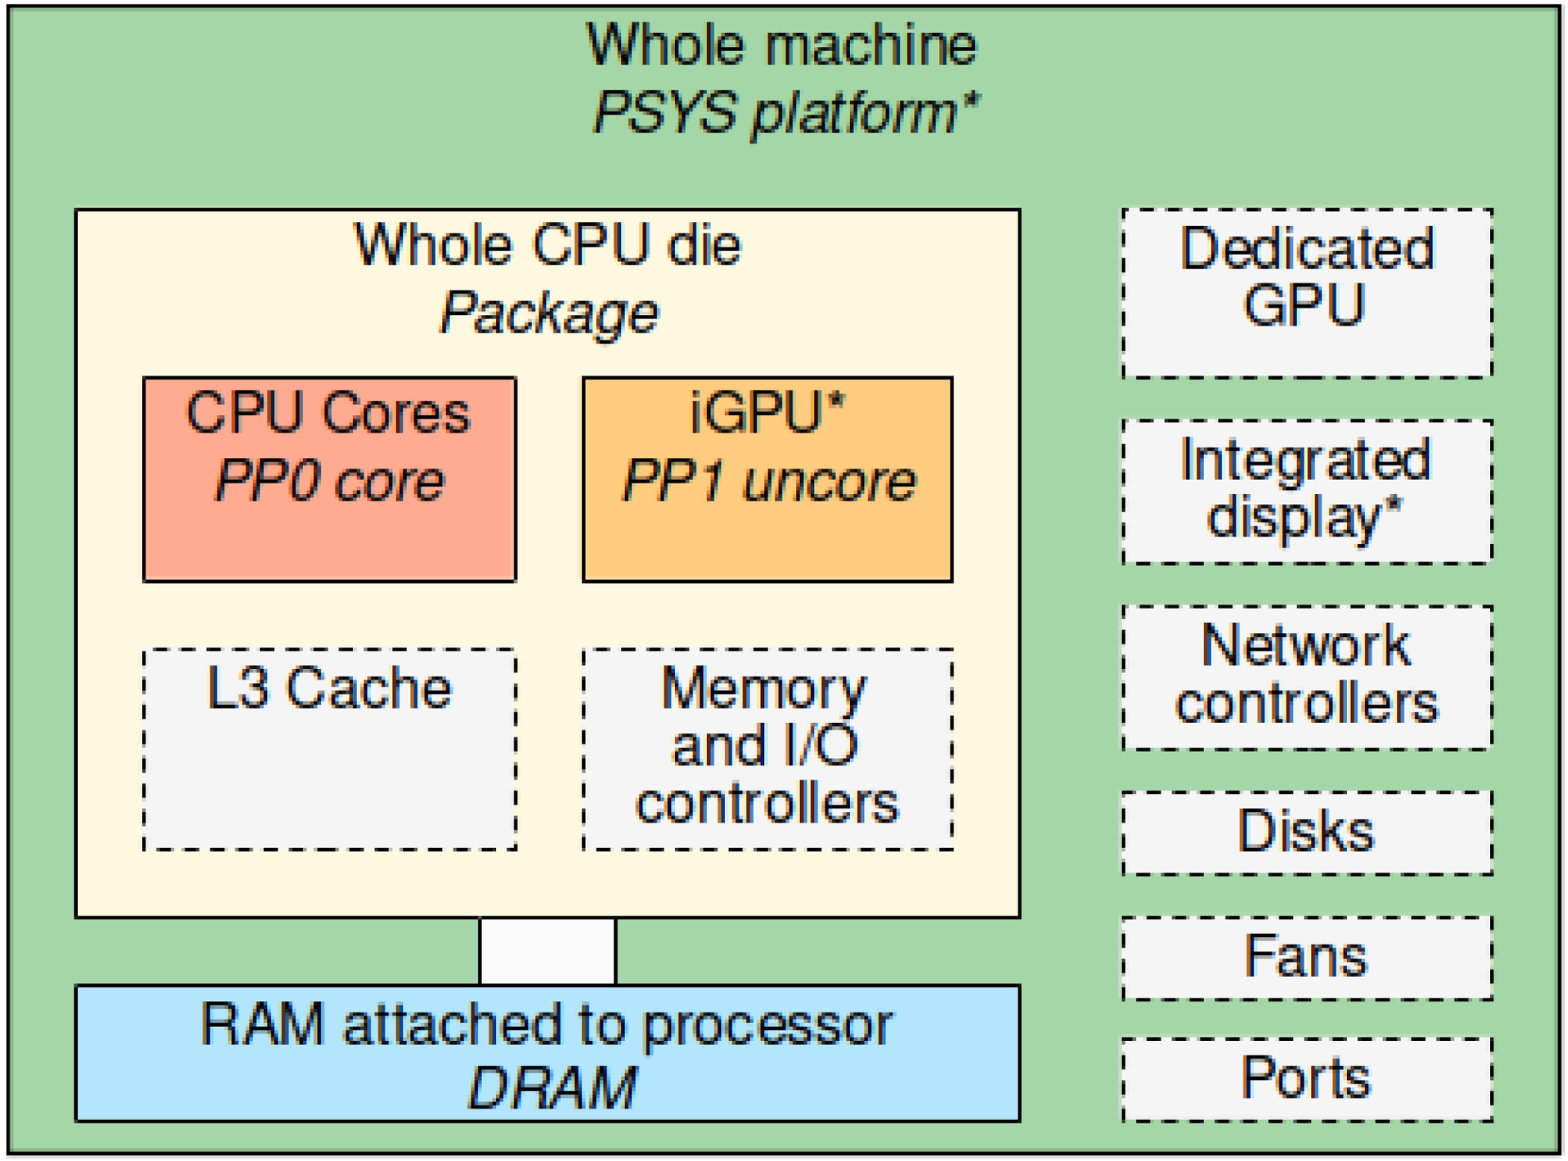
\includegraphics[width=0.7\textwidth]{Figures/rapl_domains.png}
    %\decoRule
    \caption[Rapl domains]{Hierarchy of possible RAPL domains and their corresponding hardware components. Domain names are in italic, and grayed items do not form a domain on their own, items with an asterisk are not present on servers\parencite{raffin2024dissecting}.}
    \label{fig:rapl_domains}
\end{figure}

RAPL provides hardware counters to read the energy consumption (and set power limits) for each domain. The energy consumption is measured in terms of processor-specific "energy units" (e.g. 61$\mu$J for Haswell and Skylake processors). The counters are exposed to the operating system through model-specific registers (MSRs) and are updated approximately every millisecond. The main advantages of RAPL are that no external powermeters are required, nor a privileged access to the BMC (which could be used to power off the server). RAPL is more accurate than any untuned statistical estimation model.

Various measurement methods can be used to extract RAPL measurements. In a detailed comparison, Raffin et al\parencite{raffin2024dissecting} outline their individual features and tradeoffs, which are summarize in figure~\ref{fig:rapl_interfaces_tradeoffs}:
\begin{itemize}
    \item \textbf{Lacking documentation: } Since there is no publicly available documentation of the low-level RAPL implementation, implementations are bound to suffer inaccuracies and inconsistencies due to a lack of understanding.
    \item The \textbf{Model-Specific Register (MSR)} interface provides low-level access to RAPL energy counters but is complex and hardware-dependent. Developers must manually determine register offsets and unit conversions based on processor model and vendor documentation. This method lacks safeguards, requires deep processor knowledge, and is error-prone, with incorrect readings difficult to detect. Although read-only access poses no risk to system stability, MSRs expose sensitive data and are thus restricted to privileged users (e.g., \texttt{root} or \texttt{CAP\_SYS\_RAWIO}). Fine-grained access control is not supported natively, though the \texttt{msr-safe} module offers limited mitigation.
    \item The \textbf{Power Capping (powercap)} framework is a high-level Linux kernel interface that exposes RAPL energy data through the sysfs filesystem, making it accessible from userspace. It simplifies energy measurements by automatically handling unit conversions and domain discovery, requiring minimal hardware knowledge. Though domain hierarchy can be confusing (especially with DRAM domains appearing nested under the package domain) powercap remains user-friendly and scriptable. It supports fine-grained access control via file permissions and offers good adaptability to hardware changes, provided the measurement tool doesn't rely on hard-coded domain structures.
    \item The \textbf{perf-events} subsystem provides a higher-level Linux interface for accessing RAPL energy counters as counting events. It supports overflow correction and requires less hardware-specific knowledge than MSR. Each RAPL domain must be opened per CPU socket using \texttt{perf\_event\_open}, and values are polled from userspace. While it lacks a hierarchical structure like powercap and may be harder to use in certain languages or scripts, it remains adaptable and robust across different architectures. Fine-grained access control is possible via kernel capabilities or \texttt{perf\_event\_paranoid} settings. 
    \item \textbf{eBPF} enables running custom programs in the Linux kernel, and in this context, it is used to directly read RAPL energy counters from within kernel space, potentially reducing measurement overhead by avoiding user-kernel context switches. The implementation attaches an eBPF program to a CPU clock event, using \texttt{perf\_event\_open} to access energy counters and buffering results for userspace polling (is visualized in figure~\ref{fig:rapl_perf_eBPF}).While offering the same overflow protection as regular \texttt{perf-events}, this approach is significantly more complex, prone to low-level errors (especially in C), and requires elevated privileges (\texttt{CAP\_BPF} or \texttt{root}). It also lacks portability, as it demands manual adaptation to kernel features and domain counts, limiting its maintainability across systems.
\end{itemize}
\begin{figure}[H]
    \centering
    \begin{subfigure}{0.48\textwidth}
        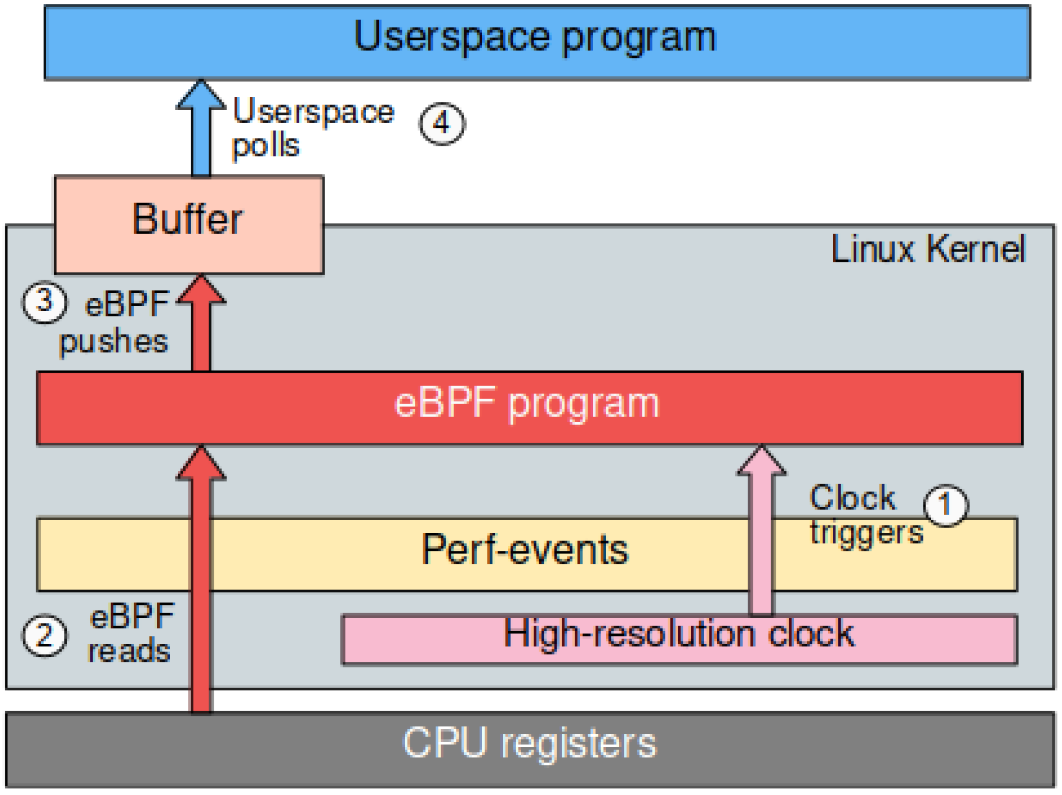
\includegraphics[width=\textwidth]{Figures/rapl_perf_eBPF.png}
        \caption[RAPL perf-event eBPF mechanism]{RAPL perf-event eBPF mechanism}
        \label{fig:rapl_perf_eBPF}
    \end{subfigure}
    \hfill
    \begin{subfigure}{0.48\textwidth}
        \vspace{1.5em}
        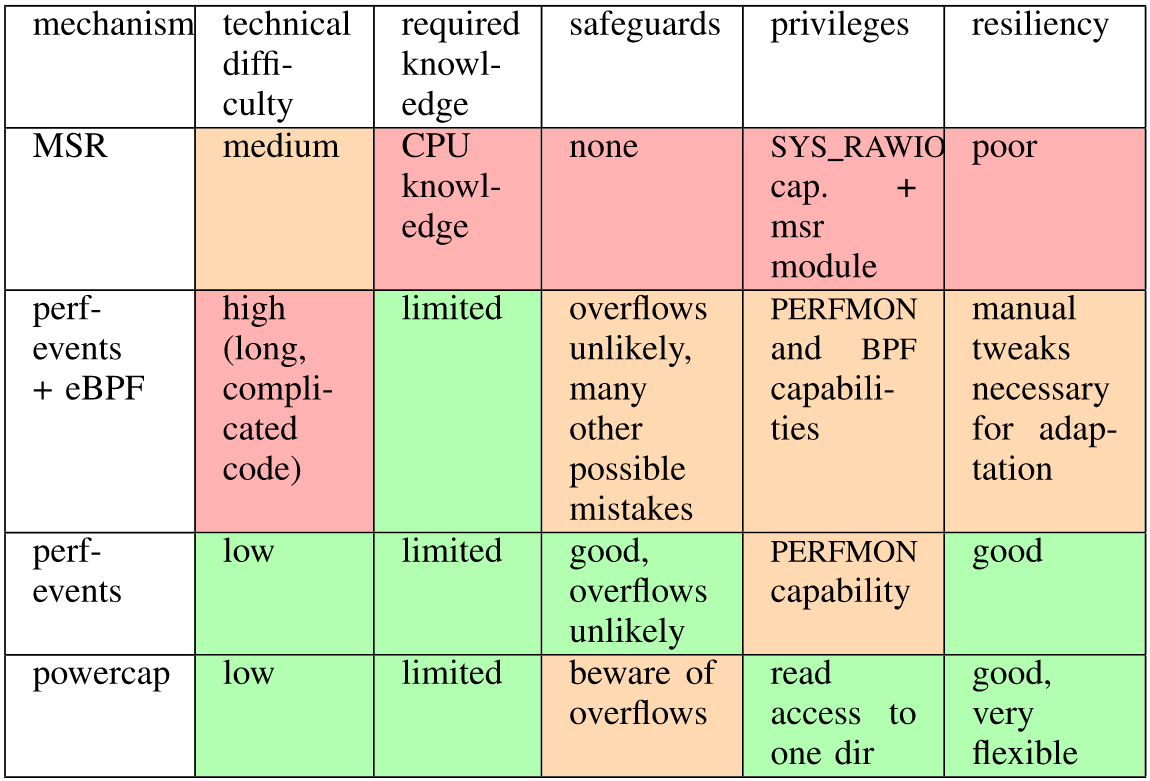
\includegraphics[width=\textwidth]{Figures/rapl_interfaces_tradeoffs.png}
        \caption[RAPL measurement mechanisms comparison]{RAPL measurement mechanisms comparison}
        \label{fig:rapl_interfaces_tradeoffs}
    \end{subfigure}
    \caption[RAPL measurements: eBPF and comparison]{RAPL measurements: eBPF and comparison\parencite{raffin2024dissecting}}
    \label{tab:measurement_mechanisms}
\end{figure}
In their research, Raffin et al conclude that all four mechanisms have small or negligible impact on the running time of their benchmarks. They formulate the following recommendations for future energy monitoring implementations:
\begin{itemize}
    \item Measuring frequencies should be adapted to the state of the node, preventing high measurement overhead, due to a reduction in time spent in low-power states. Under heavy load, a highfrequencay can be used in order to capture more information.
    \item \texttt{perf-events} is the overall recommeded measurement method with good efficiency, latency and overflow protection. Powercap is less efficient, but provides a simpler sysfs API.
    \item Even though \texttt{perf-events} and eBPF-measurement method seems to be the most energy-efficient, it is not recommended in light of its complexity. For the same reason, the MSR method is not recommeded, as it raises complexity while counter-intuitively being slower than \texttt{perf-events}
\end{itemize}

RAPL MSRs can be read on some cloud computing resources (e.g. some Amazon EC2-instances), although the hypervisor traps the MSR reads, which can add to the polling delay. in EC2, the performance overhead also significantly increases to <2.5\% (as compared to <1\% on standalone systems)\parencite{jay2023experimental}.

\subsubsection{RAPL Validation}
\label{sec:raplvalidation}
Since its inception, RAPL has been subject of various validation studies, with the general concensus that it's accuracy could be considered "good enough"\parencite{raffin2024dissecting}. Notable works are Hackenberg et al, that in 2013 found RAPL accurate but missing timestamps\parencite{hackenberg2013power}, and in 2015 noticed a major improvement to RAPL accuracy, after Intel switched from a modeling approach to actual measurements for their Haswell architecture\parencite{hackenberg2015energy}. Desrochers et al concluded in a 2016 RAPL DRAM validation study\parencite{desrochers2016validation} that DRAM power measurement was reasonably accurate, especially on server-grade CPUs. They also found measurement quality to drop when measuring and idling system. Later, Alt et al\parencite{alt2024experimental} tested DRAM accuracy of heterogeneous memory systems of the more recent Ice Lake-SP architecture and concluded that DRAM estimates behaved differently than on older architectures. They noted that the RAPL overestimates DRAM energy consumption by a constant offset, which they attribute to the off-DIMM voltage regulators of the memory system.

A critical point in the RAPL validation was the introduction of the Alder Lake architecture, marking Intel's first heterogeneous processor, combining two different core architectures from the Core and Atom families (commonly referred to as P-Cores and E-cores) to improve performance and energy efficiency. While this heterogenity can improve performance and energy efficiency, it also increases complexity of scheduling decisions and power saving mechanisms, adding to the already complex architecture, featuring per-core Dynamic Voltage and frequency Scaling (DVFS), Idle states and Power Limiting / Thermal Protection.

Schöne et al\parencite{schone2024energy} found RAPL in the Alder Lake architecture to be generally consistent with external measurements, but exhibiting lower accuracy in low power scenarios. The following figure~\ref{fig:rapl_vs_PSU_validation} shows these inaccuracies, albeit tested on a conusmer-grade Intel Core i9-12900K processor measured at the base frequency of 0.8GHz.
\begin{figure}[ht]
    \centering
    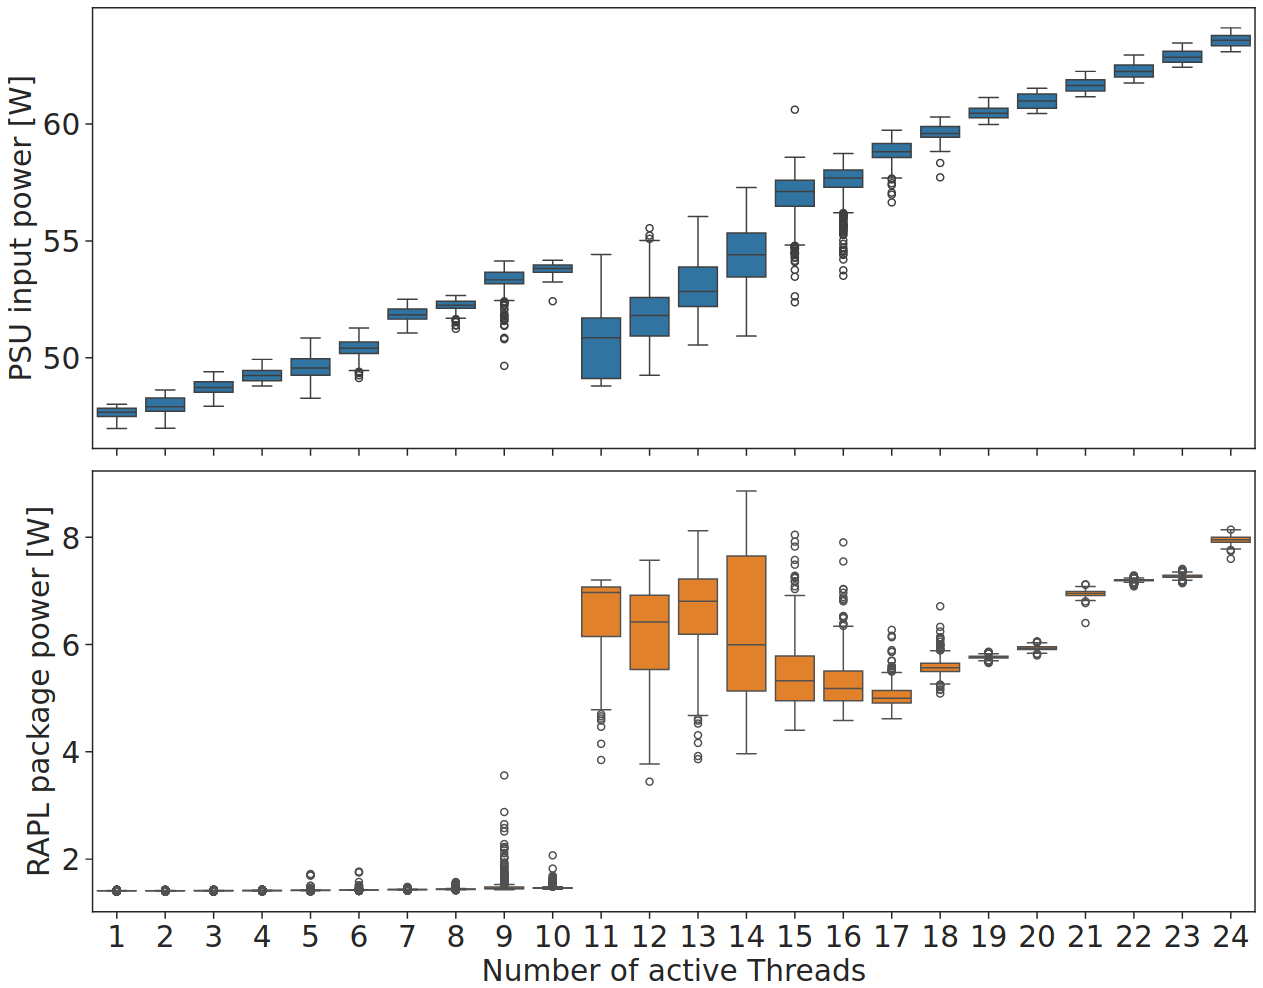
\includegraphics[width=0.7\textwidth]{Figures/rapl_vs_PSU_validation.png}
    %\decoRule
    \caption[RAPL validation: CPU vs. PSU]{RAPL and reference power consumption sampled at 100 ms / 50 ms intervals respectively. Double precision matrix multiplication kernel at 0.8GHz running for 60s each at increasing number of active threads\parencite{schone2024energy}.}
    \label{fig:rapl_vs_PSU_validation}
\end{figure}

\subsubsection{RAPL Limitations and issues}
\label{sec:rapllimitations}
Several limitations of RAPL were noticed in various research works. Since RAPL is continually improved by Intel as new Processors are released, some of these issues have since been improved or entirely solved. 

\begin{itemize}
    \item \textbf{Register overflow: }The 32-bit register can experience an overflow error\parencite{khan2018rapl, raffin2024dissecting}. This can be mitigated by sampling more frequently than the register takes to overflow. This interval can be calculated using the following equation: 
    \begin{equation}
        t_{\text{overflow}} = \frac{2^{32} \cdot E_u}{P}
    \end{equation}
    Here, $E_u$ is the energy unit used (61$\mu$J for haswell), and $P$ is the power consumption. On a Haswell processor consuming 84W, an overflow would occur every 52 minutes. Intel acknowledges this in the official documentation, stating that the register has a \textit{wraparound time of around 60 seconds when power consumption is high}\parencite{intel-sdm}
    This is solvable with a simple correction, provided that the measurement interfals are small enough: For two successive measurements $m_{\text{prev}}$ and $m_{\text{current}}$, the actual measured difference is given by
    \begin{equation}
        \Delta m =
        \begin{cases}
        m_{\text{current}} - m_{\text{prev}} + C & \text{if } m_{\text{current}} < m_{\text{prev}} \\
        m_{\text{current}} - m_{\text{prev}} & \text{otherwise}
        \end{cases}
    \end{equation}
    where C is a correction constant that depends on the chosen mechanism:
    
    \begin{table}[h]
        \small
        \begin{tabular}{|p{4cm}|p{9cm}|}
            \hline
            \textbf{mechanism} & \textbf{constant C}\\
            \Xhline{1.5pt}
            MSR & \texttt{u32::MAX} i.e. $2^{32} - 1$\\
            \hline
            perf-events & \texttt{u64::MAX} i.e. $2^{64} - 1$\\
            \hline
            perf-events with eBPF & \texttt{u64::MAX} i.e. $2^{64} - 1$\\
            \hline
            powercap & value give by the file \texttt{max\_energy\_uj} in the sysfs folder for the RAPL domain\\
            \hline
        \end{tabular}
        \caption[RAPL overflow correction constant]{RAPL overflow correction constant}
        \label{tab:RAPL_overflow_correction_constant}
    \end{table}

    \item \textbf{DRAM Accuracy: }DRAM Accuracy can only reliably be used for the Haswell architecture\parencite{desrochers2016validation, khan2018rapl, alt2024experimental}, and may still exibit a constant power offset (like attributed to the voltage regulator power loss of the memory system).
    \item \textbf{Unpredictable Timings: }While the Intel documentation states that the RAPL time unit is 0.976ms, the actual intervals may vary. This is an issue since the measurements do not come with timestamps, making precise measurements difficult\parencite{khan2018rapl}. Several coping mechanisms have been used to mitigate this, notably \textit{busypolling} (busypolling the counter for updates, significantly compromizing overhead in terms of time and energy\parencite{hahnel2012measuring}), \textit{supersampling} (lowering the sampling interval, increasing overhead and occasionaly creating duplicates that need to be filtered\parencite{khan2018rapl}), or \textit{high frequency sampling} (\textit{lowering} the sampling rate when the resulting data is still sufficient\parencite{servat2016detailed}). Another solution is to use a \textit{low sampling frequency} to smoothe out the relative error due to spikes, with the only drawback of loss of temporal precision. At sampling rates slower than 50Hz, the relative error is less than 0.5\% \parencite{jay2023experimental}.
    \item \textbf{Non-atomic register updates: } RAPL register updates are nont atomic\parencite{khan2018rapl}, meaning that the different RAPL values show a delay between individual updates. This may introduce errors when sampling multiple counters at a high sampling rate, making it possible to read both fresh and stale values of different counters.
    \item \textbf{Lower idle power accuracy: } When measuring an idling server, RAPL tends to be less accurate\parencite{schone2024energy, desrochers2016validation}.
    \item \textbf{Side-channel attacks: } While the update rate of RAPL is usually 1ms, it can get as low as 50 $\mu$s for the PP0 domain (processor cores) on desktop processors\parencite{schone2024energy}. This can be used to retrieve processed data in a side channel attack (coined "Platypus")\parencite{lipp2021platypus, schone2024energy}. 
    
    To mitigate this issue while retaining RAPL functionality, Intel implements a filtering technique via the \texttt{ENERGY\_FILTERING\_ENABLE}\parencite[Table 2-2]{intel2023} entry, or when \textit{Software Guard Extension (SGX)} is activated in the BIOS. This filter adds random noise to the reported values (vizualized in Figure~\ref{fig:rapl_platypus_filtering}). This can be seen For the PP0 domain, this raises the temporal granularity to about 8ms. While this does not affect the average power consumption, point measurement power consumption can be affected. Figure~\ref{fig:rapl_filter_granularity_loss} shows the effect of the filter, clearly indicating the loss granularity resulting from the activation of the filter. In a 2022 article, Tamara\parencite{greencoding_rapl_sgx} found a surprising higher mean with the filter activated and deemed filtered RAPL energy data unusable. In a more elaborate experiment in 2024, Schöne et al did not encounter these inaccuracies anymore.

    \begin{figure}[H]
        \centering
        \begin{subfigure}[t]{0.6\textwidth}
            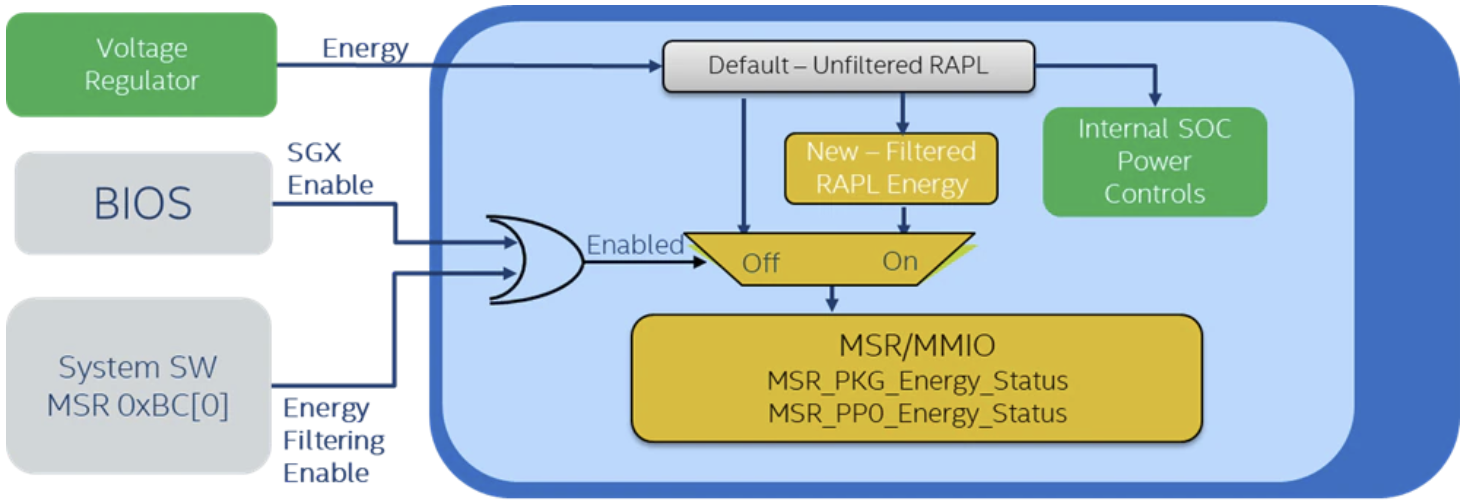
\includegraphics[width=\textwidth]{Figures/rapl_platypus_filtering.png}
            \caption{RAPL energy filtering\parencite{intel_rapl_guidance}}
            \label{fig:rapl_platypus_filtering}
        \end{subfigure}
        \begin{subfigure}[t]{0.48\textwidth}
            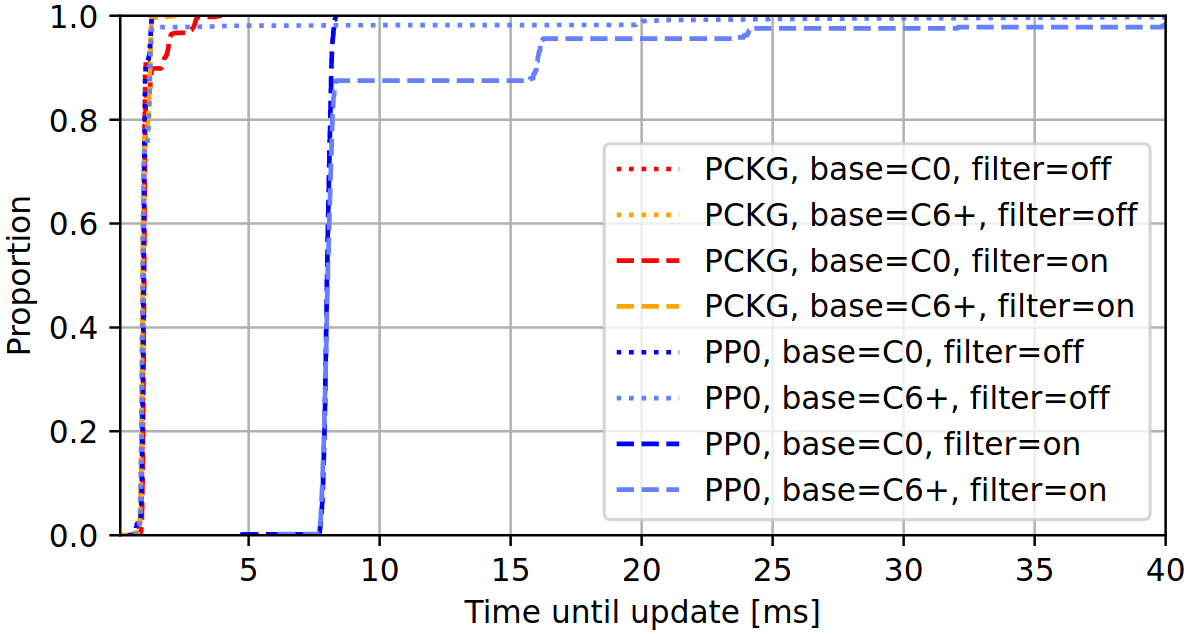
\includegraphics[width=\textwidth]{Figures/rapl_filter_granularity_loss_time.png}
            \caption{Distribution of time between updates: With an enabled filter, the PP0 domain only provides updates every 8 ms, otherwise RAPL values are updated every 1 ms. If the load is too low, some updates might be skipped, e.g., the next update for PP0 and an enabled filter is at 16 ms.}
            \label{fig:rapl_filter_granularity_loss_time}
        \end{subfigure}
        \hfill
        \begin{subfigure}[t]{0.48\textwidth}
            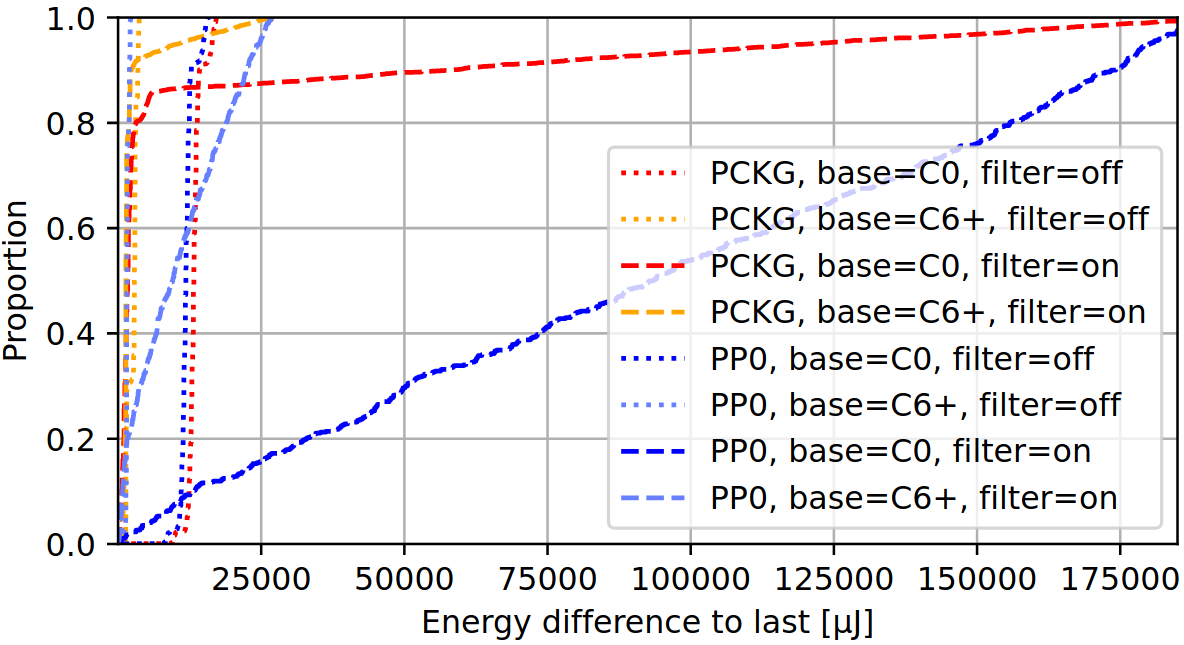
\includegraphics[width=\textwidth]{Figures/rapl_filter_granularity_loss_energy.png}
            \caption{The minimal increase of a measurement is 1 energy unit of 61.035~$\mu$J. Enabling the filter leads to a significant influence on measurements for the PP0 domain and a measurable influence on PCKG measurements.}
            \label{fig:rapl_filter_granularity_loss_energy}
        \end{subfigure}
        \caption[RAPL \texttt{ENERGY\_FILTERING\_ENABLE Granularity loss}]{Observable loss of granularity caused by the activation of \texttt{ENERGY\_FILTERING\_ENABLE}\parencite{schone2024energy}}
        \label{fig:rapl_filter_granularity_loss}
    \end{figure}
\end{itemize}

\subsubsection{RAPL conclusions}

The energy measurement accuracy of RAPl has significantly improved since its inception and provides a generally accepted way to measure system energy consumption. It is well-validated and accepted as the most accurate fine-granular energy measurement tool. Some known limitations have historically created inaccuracies in developed measurement tools, but corrections of these limitations exist. 

\subsection{Graphical Processing Units (GPU)}
In recent years, the utilization of GPUs in cloud computing environments has grown significantly, driven primarily by the increasing demand for high-performance computations in machine learning, artificial intelligence, and large-scale data processing \cite{jouppi2017datacenter}. Kubernetes now includes mechanisms for GPU provisioning, enabling containerized workloads to leverage GPU acceleration \cite{k8s_gpu_support}.

Although GPUs remain less common than traditional CPU-based workloads in typical Kubernetes clusters, their adoption is rapidly accelerating. Industry reports indicate that GPU usage in Kubernetes has seen a growth rate of nearly 58\% year-over-year, outpacing general cloud computing growth rates \cite{datadog_report}. This increase is largely attributed to ML workloads and real-time processing tasks that benefit from the parallel processing capabilities of GPUs \cite{tensorflow_k8s}. Furthermore, hyperscalers have integrated GPU support directly into their managed Kubernetes services, reflecting the growing demand for GPU-powered workloads in containerized environments.

Despite this growth, GPU deployments are still not as pervasive as CPU-based workloads in Kubernetes-managed clusters. The primary focus of this thesis is on the measurement and analysis of energy consumption in more common, CPU- and memory-centric Kubernetes workloads. Nevertheless, due to the rising significance of GPUs, their energy measurement techniques and potential integration within Kubernetes environments are briefly examined.

Ultimately, the inclusion of GPU energy measurements remains outside the primary scope of this thesis but is acknowledged as an important area for future research. This structured exploration serves to highlight current limitations and opportunities for enhancing energy efficiency in Kubernetes-managed GPU workloads.

\subsubsection{GPU virtualization technologies}

\paragraph{Full GPU Virtualization}

Full GPU virtualization provides isolated instances of a single physical GPU to multiple virtual machines. This is achieved using technologies such as NVIDIA's \textit{vGPU} or AMD's \textit{MxGPU (Multiuser GPU)}. These technologies allow a VM to see a complete GPU, while the underlying hypervisor manages resource partitioning and scheduling \cite{nvidia_virtualization, amd_instinct_virtualization} eigher though the use of partitioning or time-slicing. In a Kubernetes environment, full GPU virtualization is commonly utilized through:
\begin{itemize}
    \item \textbf{vGPU on VMware or OpenStack:} Kubernetes clusters running on VMware vSphere or OpenStack can request vGPU instances as if they were physical GPUs. These instances are shared among containers while maintaining memory and compute isolation.
    \item \textbf{Device Plugin Integration:} NVIDIA, AMD and Intel provide a Device Plugin for Kubernetes, enabling seamless GPU discovery and allocation across pods \cite{k8s_gpu_support}.
\end{itemize}

\paragraph{Multi-Instance GPU (MIG)}
Introduced with the NVIDIA A100 architecture, Multi-Instance GPU (MIG) allows a single GPU to be partitioned into up to seven independent instances, each with its own dedicated compute, memory, and cache resources \cite{nvidia_mig_user_guide}. Unlike traditional vGPU, MIG provides true hardware-level isolation, preventing noisy-neighbor effects and enabling finer resource allocation. MIG instances are exposed to Kubernetes as individual GPUs. For example, a single A100 GPU partitioned into seven MIG instances appears as seven separate GPU resources, each assignable to different containers. MIG-aware device plugins ensure proper scheduling and isolation. Hence, MIG technology is particularly useful for multi-tenant environments and supports finer granularity in resource allocation compared to traditional vGPU models.

\paragraph{GPU Passthrough}
GPU passthrough allows a physical GPU to be exclusively assigned to a single VM or container. Unlike virtualization, where resources are shared, passthrough dedicates the full GPU to one environment, offering near-native performance \cite{nvidia_passthrough}. GPU passthrough is configured at the hypervisor level (e.g., KVM or VMware ESXi) and can be exposed to Kubernetes nodes. Pods scheduled on nodes with GPU passthrough access gain complete control of the GPU, enabling direct memory access and high-performance computation.

GPU virtualization technologies enable efficient multi-tenant use of GPU resources, enhancing performance and cost-effectiveness in cloud-native environments. For the purposes of energy measurement, understanding these virtualization layers is essential for accurate per-container energy attribution.

\subsubsection{GPU nvidia-NVML energy measurements and validation}

Modern GPUs are equipped with \textbf{built-in power sensors} that enable real-time energy measurement. For instance, Nvidia GPUs expose power metrics through the \textit{Nvidia System Management Interface (nvidia-smi)}, which reports instantaneous power draw, temperature, and memory usage \cite{nvidia_smi_docs}. This interface allows for programmatic access to GPU power consumption, making it a common choice for monitoring and energy profiling in both standalone and containerized environments \cite{nvidia_mig_user_guide}.

In 2024, Yang et al. conducted a comprehensive study on the accuracy and reliability of NVIDIA's built-in power sensors, examining over 70 different models\cite{yang2024accurate}. He concludes that previous research placed excessive trust in nvidia-NVML, overlooking the importance of measurement methodology. The study revealed several critical findings:
\begin{itemize}
    \item \textbf{Sampling Limitations:} Nvidia NVML gives the option to specify a sampling frequency in units of milliseconds. However, on certain models, such as the A100 and H100, power is sampled only around 25\% of the time, introducing potential inaccuracies in total energy consumption estimations.
    \item \textbf{Transient Response Issues:} While measured power reacted instantly to a suddenly applied workload, nvidia-NVML would report values with a delay of several hunderd milliseconds on some devices. Also, a slower rise (with linear growth) was discovered, taking over a second to catch up to correct power figures in some instances. Generally, server-grade GPUs were shown to provide more instantaneous power measurements.
    \item \textbf{Measurement Inaccuracies:} The average error rate in reported power draw was found to be approximately 5\%, deviating from NVIDIA's claimed fixed error margin of 5W. This error would remain consistent when the GPU reached a constant power draw.
    \item \textbf{Averaging Effects:} Reported power consumption values are averaged over time, masking short-term fluctuations and potentially underreporting peak consumption.
\end{itemize}

To address these limitations, the study proposed best practices such as running multiple or longer iterations of workloads to average out sampling errors, introducing controlled phase shifts to capture different execution states, and applying data corrections to account for transient lags \cite{yang2024accurate}. These adjustments reduced measurement errors by up to 65\%, demonstrating the importance of refining raw sensor data for more accurate energy profiling.

\subsubsection{Related Research}
While most reaseach has used nvidia-NVML to measure GPU power consumption, some research was done on alternative measurement tools, ususally to address similar issues as were stated by Yang et al in the previous section. Specifically, the following three tools focussed were proposed to provide higher sampling rates to enable finer-grained power analysis.
\paragraph{AccellWattch}
In 2021, Pan et al proposed \textit{AccelWattch}\parencite{kandiah2021accelwattch}, a configurable GPU power model that provides both a higher accuracy cycle-level power model, and a way to measure constant and static power, utilizing any pure-software software performance mode,nvidia-NVML, or a combination of the two. Notably, their model is DVFS-, power-gating- and divergence-aware. The resulting power model was validated against measured ground truth using an Nvidia Volta GV100, yielding a MAPE error between $7.5-9.2 \pm 2.1\%-3.1\%$, depending on the AccelWattch variant. The Volta model was later validated against Pascal TITAN X and Turing RTX 2060-architectures without retraining, achieving $11 \pm 3.8\% and 13 \pm 4.7\%$ MAPE, respectively. The authors conclude that AccelWattch can reliably predict power consumption of these specific GPU architectures. In the context of Kubernetes energy consumption, AccelWattch contributes a fine-grained temporal granularity

\paragraph{FinGraV}
In 2024, Singhania et al propose \textit{FinGraV}\parencite{singhania2024methodology} (abbreviated from \textbf{Fin}e-\textbf{Gra}in \textbf{V}isibility), a fine-grained power measurements tool capable of sub-millisecond power profiling for GPU executions on an AMD MI300X GPU. They identify these main challenges of high-resolution GPU power analysis (see figure~\ref{fig:fingrav_challenges}):
\begin{itemize}
    \item \textbf{Low sampling frequency:} Standard GPU power loggers operate at intervals too coarse (tens of milliseconds) to capture the sub-millisecond executions of modern kernels.
    \item \textbf{CPU-GPU time Synchronization:} Synchronizing power measurements with kernel start and end times is problematic due to the asynchronous nature of CPU-GPU communication.
    \item \textbf{Execution time variation:} Minor variations in memory allocation or access patterns lead to inconsistent kernel execution times, complicating time-based power profiling.
    \item \textbf{Power variance across executions:} Repeated executions of the same kernel, or interleaved executions with other kernels, manifest in fluctuating power consumption, challenging consistent profiling.
\end{itemize}

\begin{figure}[H]
    \centering
    \begin{subfigure}{1\textwidth}
        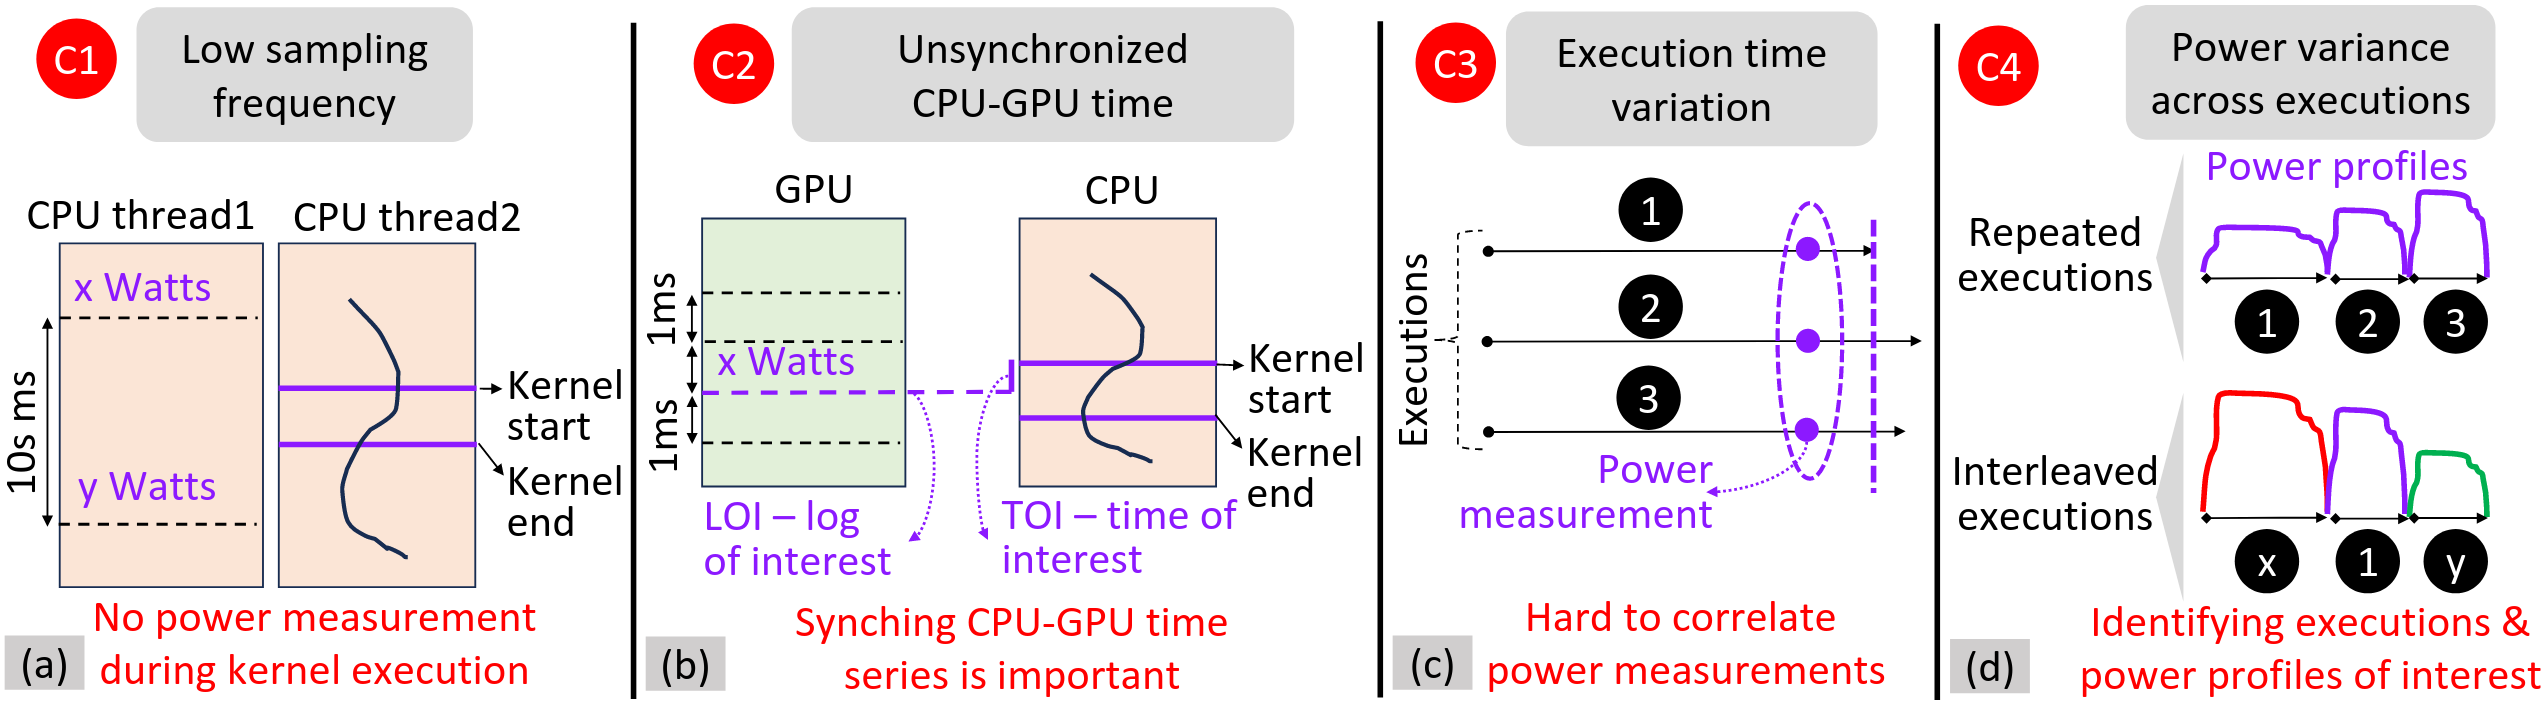
\includegraphics[width=1\textwidth]{Figures/fingrav_challenges.png}
        \caption[Challenges in fine-grain GPU power analysis]{Challenges in fine-grain GPU power analysis}
        \label{fig:fingrav_challenges}
    \end{subfigure}
    \hfill
    \begin{subfigure}{1\textwidth}
        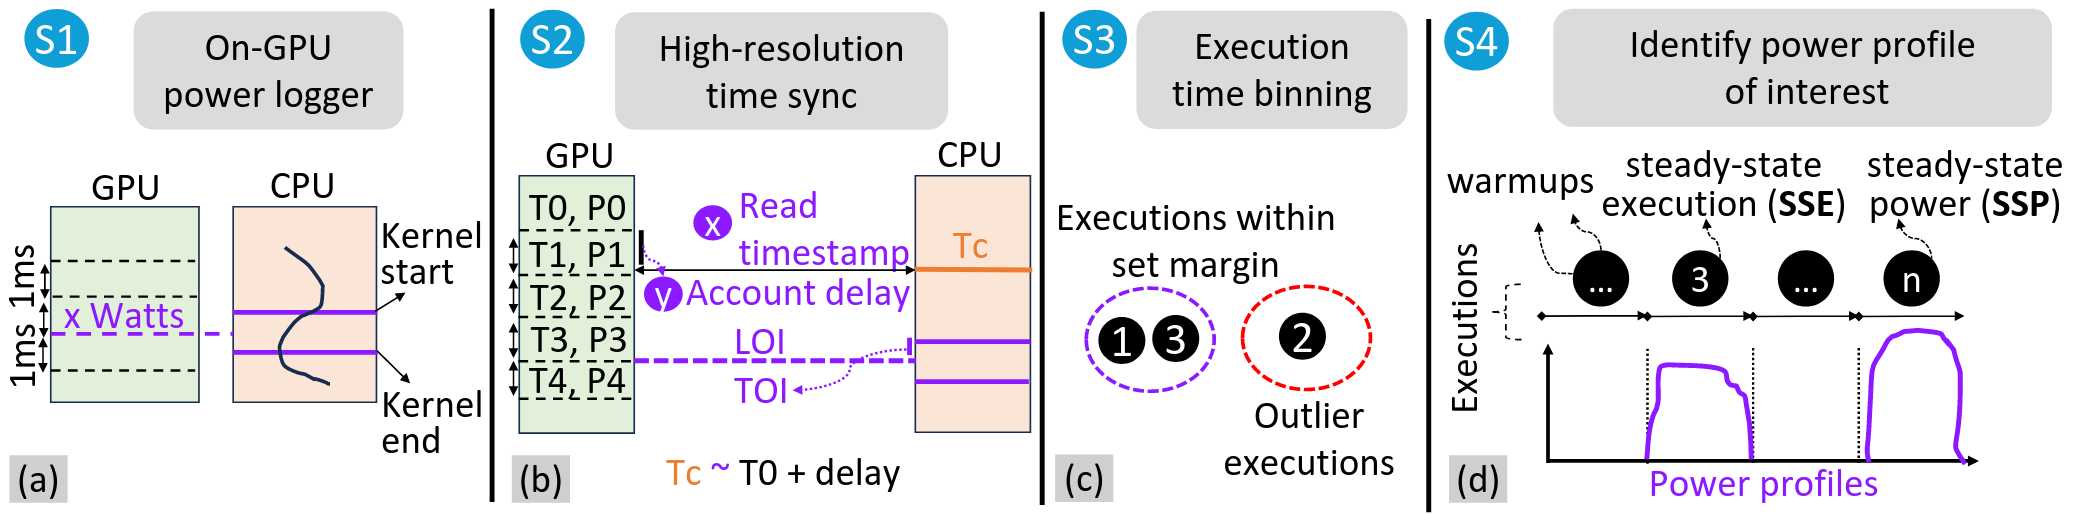
\includegraphics[width=1\textwidth]{Figures/fingrav_solutions.png}
        \caption[FinGraV strategies to adress challenges]{FinGraV strategies to adress challenges}
        \label{fig:fingrav_solutions}
    \end{subfigure}
    \caption[FinGraV GPU power measurement challenges and strategies]{FinGraV GPU power measurement challenges and strategies\parencite{singhania2024methodology}}
    \label{fig:fingrav_challenges_solutions}
\end{figure}

To overcome these challenges, FinGraV introduces several strategies (see figure ~\ref{fig:fingrav_solutions}). 
\begin{itemize}
    \item \textbf{On-GPU Power Logger:} FinGraV leverages a high-resolution (1 ms) power logger, capturing the average of multiple instantaneous power readings.
    \item \textbf{High-Resolution Time Synchronization:} GPU timestamps are read from the CPU side before kernel execution, and synchronization is maintained throughout execution to correlate power samples with kernel events.    
    \item \textbf{Execution Time Binning:} Kernel executions are grouped into "bins" based on empirical runtime ranges, enabling tighter power profiling while discarding outlier runs.    
    \item \textbf{Power Profile Differentiation:} FinGraV distinguishes between Steady-State Execution (SSE) and Steady-State Power (SSP) profiles. SSP represents the stabilized power consumption after initial transients, providing the most accurate depiction of kernel power consumption.
\end{itemize}
The application of FinGraV to bencharmks reveals several critical obervations: Kernel executions differ significantly between initial runs and steady-state, with deviations up to 80\%. Memory-bound kernels and compute-light kernels are found to be highly sensitive to the preceding kernel, impacting their power profile. Furthermore, the authors expose discrepancies in GPU power scaling relative to computational load, particularly for compute-light kernels.

FinGraV introduces promising concepts that could, in theory, enable more granular and accurate GPU power analysis in container-based GPU workloads. Its methodological approach addresses key challenges in sub-millisecond power measurement. However, its current implementation is tightly coupled with the AMD MI300X GPU, relying on hardware-specific logging capabilities that are not universally available. While the underlying concepts may be extendable to other GPUs, achieving this is far from trivial, requiring significant adaptation and low-level access to power metrics that are often proprietary or limited by driver capabilities.

Consequently, FinGraV highlights both the challenges and potential solutions for fine-grained GPU power analysis but falls short of providing a general-purpose framework that could be easily integrated into Kubernetes energy measurement tools. It also underscores the broader issue that GPU energy consumption analysis remains relatively immature, with only vendor-specific tools like nvidia-NVML offering practical—albeit coarse—power metrics. This illustrates that while the methodology is theoretically sound, practical implementation across diverse GPU architectures remains a significant challenge.

\paragraph{PowerSensor3}
\textit{PowerSensor3}\parencite{van2025powersensor3} is an open-source hardware tool introduced in 2025, designed to provide high-resolution power measurements for GPUs, SoC boards, PCIe devices, SSDs, and FPGAs. Unlike software-based power models or vendor-specific tools such as NVIDIA's NVML, PowerSensor3 achieves significantly higher accuracy and granularity through direct voltage and current measurements at a sampling rate of up to 20 kHz. This fine temporal resolution allows it to capture transient power behaviors that are typically missed by software-based methods, which are constrained by lower sampling frequencies and indirect estimations. As expected for a purpose-built hardware solution, PowerSensor3 outperforms NVML in both precision and the ability to detect rapid changes in power consumption.

A particularly valuable feature of PowerSensor3 is its capability to monitor not only GPUs but also other critical components such as SoC boards, PCIe-connected accelerators, and storage devices like SSDs. For Kubernetes-based energy efficiency analysis, this would provide unprecedented visibility into the power usage of individual containers, extending monitoring beyond the CPU and GPU to the broader spectrum of peripherals that contribute to overall energy consumption. Such granularity could enhance resource scheduling and energy optimization in containerized environments.

However, while its technical benefits are evident, the practical deployment of dedicated hardware sensors like PowerSensor3 at scale remains both complex and expensive. Integrating such devices across large Kubernetes clusters would require substantial investment in hardware and reconfiguration of infrastructure, making wide adoption unlikely outside of specialized research environments. Consequently, PowerSensor3 and other hardware-dependent methods are not considered in the scope of this thesis. Furthermore, the very recent introduction of PowerSensor3 in 2025 highlights the ongoing challenges of accurate energy monitoring through software alone, reflecting the current gap in reliable, scalable, software-based power measurement solutions.

\subsubsection{GPU Limitations in Kubernetes Context}
The analysis of GPU power consumption has revealed promising research efforts aimed at achieving fine-grained power visibility and energy optimization. Tools such as FinGraV and PowerSensor3 demonstrate that significant strides are being made in capturing detailed power metrics with high temporal resolution and sub-component granularity. FinGraV addresses the complexities of short-lived GPU kernel executions through innovative profiling methodologies, while PowerSensor3 delivers hardware-level accuracy for GPUs, SoC boards, and various PCIe-connected peripherals. These solutions underscore the potential for more refined power monitoring in high-performance GPU workloads.

However, the current state of GPU energy consumption measurement presents significant challenges for scalable, container-based energy tracking in Kubernetes environments. Research tools like FinGraV and PowerSensor3, while technically robust, are either hardware-dependent or too tightly coupled to specific architectures—such as AMD's MI300X in the case of FinGraV. Hardware-based solutions like PowerSensor3, though highly accurate, are impractical for widespread deployment due to cost and scalability concerns. Meanwhile, software-based vendor solutions such as NVIDIA's NVML are far more accessible, but suffer from limitations in temporal granularity and measurement accuracy. These tools offer convenient integration and broad support across data center infrastructures but struggle with capturing rapid transients in power consumption, which are crucial for real-time container energy attribution. 

In the context of this thesis, GPU energy consumption is acknowledged as an important yet currently impractical aspect of container energy measurement. The relative immaturity of fine-grained, scalable monitoring solutions for GPUs, combined with the relatively small role of GPUs in Kubernetes clusters, justifies this exclusion. Although the utilization of GPU accelerators in Kubernetes environments is expected to grow, current measurement methods do not yet support the level of precision and scalability required for effective implementation. As such, this thesis will focus on more readily measurable server components, with the understanding that future advancements in GPU power analysis may enable their integration into Kubernetes-based energy efficiency strategies.

\subsection{Storage Devices}
Various sudies have investigated the power consumption of Storage devices. In 2008, Hylick et al\parencite{hylickAnalysisHardDrive2008a} investigated real-time HDD energy consumption and found significant differences in power consumption between standby, idle and active power states. Cho et al\parencite{choDesignTradeoffsSSDs2015} propose various energy estimation models for SSDs after measuring and comparing the energy consumption of different models. The most notabble model-based energy consumption estimation methanisms are presented in section~\ref{sec:model-based_storage_power}

In constrast to CPU or GPU components, storage devices (HDD, DDS or NVMe-drives) cannot make use of physical power sensors. While a BMC-measurement-based solution would technically be feasable, real-world implementation is impractical: While a BMC might me able to measure the power supply to a storage device, it typically is not exposed through IPMI or redfish. Such measurements would further be compllicated by the use of backplane devices, making measurements for individual devices impossible. For these reasons, storage device energy consumption is typically modelled, not measured (see section ~\ref{sec:storageModeling}).

While storage devices don't expose any energy-consumption specific metrics, many other related metrics are available (and can be used for modeling approaches):
\begin{itemize}
    \item \texttt{NVMe-cli}\parencite{nvmecli_github} exposes many metrics of NVMe-drives, including the maximum power draw for each power state (including idle power), the number of power states supported, the current power state and temperature, and others.
    \item \texttt{smartctl}\parencite{smartmontools_github} exposes metrics of the \textit{SMART (Self-Monitoring, Analysis and Reporting Technology)}-Functionality implemented in many modern storage drives. While these metrics are vendor-specific, they often include temperature metrics, throughput, and other metrics. Often, HDD speed is exposed. Notably, \textit{SMART} metrics are typically more focussed on lifecycle information such as power-on hours, wear indicators and others.
    \item Many other performance metrics are exposed by various tools such as \texttt{iostat}, \texttt{sar}, \texttt{/proc/diskstats}, and \texttt{blkstat}, such as read/write IOPS, throughput, queue length, latency, utilization, and others. Additional information (such as the interface) is also exposed.
\end{itemize}











\section{Model-based estimation techniques}
In the absence of actual power data, power consumption models can be formulated that essentially map variables (such as CPU, Memory utilization) related to a server's state to its power consumption. 
Due to the strong correlation between CPU uzilization and server power, a great number of models use CPU metrics as the only indicator of server power. Fan et al\parencite{fan2007power} proposed a linear interpolation between idle power and full power, which they further refine into a non-linear form, with a parameter $\gamma$ to be fitted to minimize mean square error. Similar research was done to further reduce error by introducting more complex non-linear models, such as Hsu and Poole\parencite{hsu2011power}, who studied the SPECpower\textunderscore ssj2008-dataset of systems released between December 2007 and August 2010, and suggested the adaptation of two non-linear terms:
\begin{equation}
    P_{\text{server}} = \alpha_0 + \alpha_1 u_{\text{cpu}} + \alpha_2 \left( u_{\text{cpu}} \right)^{\gamma_0} + \alpha_3 \left( 1 - u_{\text{cpu}} \right)^{\gamma_1}
\end{equation}

While models like these might work well when custom-fitted to specific, multi-purpose servers, they have since been surpassed by the more common approach of modelling server power is to consider it an assembly of its components, such as Song et al\parencite{song2013unified} propose as:
\begin{equation}
    P_{\text{server}} = P_{\text{cpu}} + P_{\text{memory}} + P_{\text{disk}} + P_{\text{NIC}} + C
\end{equation}
, where C denotes the server's base power, which includes the power consumption of other components (regarded as static). This approach can easily be extended to include various other components such as GPUs, FPGAs or other connected components.


....

general issue \parencite{lin2020taxonomy}: There have been extensive studies on hardware-centric power models. However, it can be observed that the interactions between the components are not considered in most research at either the machine level or the component level. Considering the complexity of the workload on a cloud server, it is necessary to investigate the correlation between the power consumption of different components and take that into account. For example, the power characteristic of the CPU could be entirely different in memory-intensive (while low disk usage) jobs and in IO-intensive jobs.


\subsection{Model-based estimation techniques for storage devices}
\label{sec:model-based_storage_power}

\subsubsection{Generalization-based estimation}
There is an urgent need in the storage industry for research into the area of workload-dependant power estimation\parencite{allaloufStorageModelingPower2009}. Estimating the energy consumption of a storage device is challenging especially due to the great variation between different devices. Some of these model variables can be determined on a running server system (e.g. device type, I/O operation type, access pattern, workload intensity, state and more), while other variables are unknown to the server (e.g. Flash Transition Layer and flash factor, NAND organization, garbage collection, and more). A large storage device market has led to a high variation in devices with sometimes drastically different target uses (e.g. low-latency storage devices, high-concurrency storage devices, low-power storage devices).

Storage controllers further complicate the energy consumption estimation of storage devices by introducing an additional layer of abstraction between the operating system and the physical storage hardware. Their internal operations consume energy independently of the actual read/write workload observed by the host system. This makes it difficult to directly correlate application-level I/O activity with actual device-level power usage. Moreover, in many server configurations, multiple drives are managed behind a single controller, obscuring per-device energy attribution and introducing variability that model-based estimations often cannot accurately capture.

\paragraph{Scope clarification} 
In this thesis, only storage devices physically installed in the server are considered for power estimation. This includes devices such as HDDs, SSDs, and NVMe drives directly attached to the server. Dedicated external storage systems such as Storage Area Networks (SAN) or Network-Attached Storage (NAS) are not within the scope of this analysis. While such systems are important in data center environments, their energy consumption is not attributable at the granularity required for the workload-level estimation pursued in this thesis.

As a result, research into storage device energy consumption measurement that is generally applicable to all devices has been limited. For practical applications, generalizations are often used, such as the following tables~\ref{tab:Storage_power_HDD} to~\ref{tab:Storage_power_NVMe}. While these approximations cannot be used in the context of this thesis, they may serve as an initial guideline.

\begin{table}[H]
    \centering

    \begin{subtable}[t]{\textwidth}
        \centering
        \begin{tabular}{ |c|c|c|c| } 
            \hline
            \textbf{HDD Type} & \textbf{Read/write power (W)} & \textbf{Idle Power (W)} & \textbf{Standby Power (W)} \\
            \Xhline{1.5pt}
            HDD (2.5'' SATA) & 1.5 -- 3.0 & 0.5 -- 1.2 & 0.1 -- 0.3 \\
            \hline
            HDD (3.5'' SATA) & 6 -- 12 & 4 -- 8 & 0.5 -- 2.0 \\
            \hline
            HDD (Enterprise) & 7 -- 15 & 5 -- 10 & 0.5 -- 2.5 \\
            \hline
        \end{tabular}
        \caption[Typical HDD power consumption]{Typical HDD power consumption\parencite{storedbits_hdd}}
        \label{tab:Storage_power_HDD}
    \end{subtable}

    \vspace{1em}

    \begin{subtable}[t]{\textwidth}
        \centering
        \begin{tabular}{ |c|c|c|c| } 
            \hline
            \textbf{HDD Type} & \textbf{Read/write power (W)} & \textbf{Idle Power (W)} & \textbf{Standby Power (W)} \\
            \Xhline{1.5pt}
            5400 RPM HDD & 6 -- 9 & 4 -- 6 & 0.5 -- 1.5 \\
            \hline
            7200 RPM HDD & 8 -- 12 & 6 -- 8 & 0.6 -- 1.8 \\
            \hline
            10,000+ RPM HDD & 10 -- 16 & 8 -- 12 & 1.0 -- 2.5 \\
            \hline
        \end{tabular}
        \caption[Common HDD RPM power consumption]{Common HDD RPM power consumption\parencite{storedbits_hdd}}
        \label{tab:Storage_power_HDD_RPM}
    \end{subtable}

    \vspace{1em}

    \begin{subtable}[t]{\textwidth}
        \centering
        \begin{tabular}{ |c|c|c|c| } 
            \hline
            \textbf{SSD Type} & \textbf{Read Power (W)} & \textbf{Write Power (W)} & \textbf{Idle Power (W)} \\
            \Xhline{1.5pt}
            2.5'' SATA & 4.5 -- 8 & 4.5 -- 8 & 0.30 -- 2 \\
            \hline
            mSATA & 1 -- 5 & 4 -- 8 & 0.20 -- 2 \\
            \hline
            M.2 SATA & 2.5 -- 6 & 4 -- 9 & 0.40 -- 2 \\
            \hline
        \end{tabular}
        \caption[Typical SATA SSD power consumption]{Typical SATA SSD power consumption\parencite{storedbits_ssd}}
        \label{tab:Storage_power_SSD}
    \end{subtable}

    \vspace{1em}

    \begin{subtable}[t]{\textwidth}
        \centering
        \begin{tabular}{ |c|c|c|c| } 
            \hline
            \textbf{NVMe Type} & \textbf{Read/write power (W)} & \textbf{Peak Power (W)} & \textbf{Standby Power (W)} \\
            \Xhline{1.5pt}
            M.2 NVMe PCIe 3.0 & 3 -- 5 & 6 -- 9 & 0.4 -- 1.5 \\
            \hline
            M.2 NVMe PCIe 4.0 & 5 -- 7 & 8 -- 12 & 0.5 -- 2 \\
            \hline
            M.2 NVMe PCIe 5.0 & 8 -- 12 & 12 -- 18 & 0.8 -- 3 \\
            \hline
        \end{tabular}
        \caption[Typical NVMe SSD power consumption]{Typical NVMe SSD power consumption\parencite{storedbits_ssd}}
        \label{tab:Storage_power_NVMe}
    \end{subtable}

    \caption[Power consumption for storage types]{Power consumption for various storage device types.}
    \label{tab:Storage_power_grouped}
\end{table}

Apart from simple estimations like shown in tables~\ref{tab:Storage_power_HDD} to ~\ref{tab:Storage_power_NVMe}, a few works have concentrated on the energy consumption of individual storage devices. In 2015, Cho et al developed Energysim\parencite{choDesignTradeoffsSSDs2015}, an SSD energy modeling framework avancing the understanding of component-level (i.e. the subcomponents of a storage device) energy consumption in storage devices. Its validation against real-world SSD measurements against an Intel X25-M yielded a less than 8\% error. The work underscores the difficulty of modeling storage energy accurately due to high variability across architectures and workloads. Unfortunately, Energysim uses many model parameters such as NAND organization, idle and active current consumption, and as a result cannot reneralized to other storage devices where these are unknown.

In 2014, Li and Long\parencite{liWhichStorageDevice2014} present a workload-aware modeling framework to estimate the energy consumption of storage systems, challenging the assumption that SSDs are inherently more energy-efficient than HDDs. By classifying I/O workloads into capability workloads (performance-driven) and capacity workloads (storage size-driven), they develop mathematical models that account for the number of devices needed, workload execution time, and device power states (active, idle, standby). Their validation, based on empirical measurements using Seagate HDDs and a Samsung SSD, shows that SSDs are generally more efficient for high-performance workloads, while HDDs can outperform SSDs in archival or low-access scenarios—particularly when effective power management (e.g., spin-down) is employed. Unfortunately, similar to the research by Cho et al, the presented models make use of various non-generalizable variables, most notably a devices idle, standby and busy power consumption. In the context of these thesis, these are unknown and the presented model consequently cannot be applied.

\subsubsection{GSPN Modeling for hybrid storage systems (active power states)}
In 2022, Borba et al\parencite{borbaModelingApproachEstimating2022} proposed a number of models based on generalized stochastic Petri nets (GSPN) for performance and energy consumption evaluation for individual and Hybrid (HDD + SSD) storage systems. GSPN is a suitable formalism for storage system design, as, differently from queueing network models (for instance), synchronization, resource sharing, and conflicts are naturally represented. Also, phase approximation technique may be applied for modeling non-exponential activities, and events with zero delays (e.g., workload selection) may adopt immediate transitions. 

The authors propose a single-storage model (either for a single storage device or a hybrid system as a blackbox) and a multiple storage model.

The Hybrid storage power consumption model proposed by Borba is parameterized by I/O type (read/write), access pattern (sequential/random), object size (4KB, 1MB), and thread concurrency. The model explicitely imcorporates power consumption per operation (e.g. random-read-4KB on SSD).

The following notation is adoped:
\begin{itemize}
    \item $E\{\#p\}$ represents the mean value of the inner expression, in which $\#p$ denotes the number of tokens in place.
    \item $W(T)$ represents the firing rate associated with transition $T$.
    \item $\eta : T_{\text{imm}} \rightarrow [0, 1]$ maps each immediate transition ($t \in T_{\text{imm}}$) to a normalized weight. Weights represent the transition firing probablilty in a conflict set.
    \item $pRequests(N)$ denotes the amount of concurrent requests from simultaneous clients (workers)
\end{itemize}

Single-device storage energy consumption is estimated as follows:
\begin{align}
    EP_w = \kappa \cdot (&EP_{w1} \cdot \alpha \cdot \beta 
        + EP_{w2} \cdot (1 - \alpha) \cdot \beta \notag \\
        &+ EP_{w3} \cdot \alpha \cdot (1 - \beta) 
        + EP_{w4} \cdot (1 - \alpha) \cdot (1 - \beta))
\end{align}
\begin{align}
    EP_r = (1 - \kappa) \cdot (&EP_{r5} \cdot \alpha \cdot \beta 
        + EP_{r6} \cdot (1 - \alpha) \cdot \beta \notag \\
        &+ EP_{r7} \cdot \alpha \cdot (1 - \beta) 
        + EP_{r8} \cdot (1 - \alpha) \cdot (1 - \beta))
\end{align}
\begin{equation}
    EC = (EP_w + EP_r) \cdot TH \cdot \text{time}
\end{equation}
where $EP_w$ and $EP_r$ are the mean power consumption for a read ($r$) or write ($w$) operation, which is estimated using the mean power of each workload feature. For instance, $EP_{w1}$ denotes the power of a write operation ($w$) using random access ($\alpha$) and a small object ($\beta$). System throughput (i.e., IOPS) is estimated as $TH = E\{\#p_{\text{Ack}}\} \times W(t_{\text{Communicating}})$.For the single device model, the following weights are taken into account:
$\eta(t_{\text{Write}}) = \kappa$;  
$\eta(t_{\text{Read}}) = 1 - \kappa$;  
$\eta(t_{\text{Random}}) = \alpha$;  
$\eta(t_{\text{Sequential}}) = 1 - \alpha$;  
$\eta(t_{\text{Small}}) = \beta$; and  
$\eta(t_{\text{Large}}) = 1 - \beta$.

The marking of place $pResource (R)$ (for both read or write activity) may denote the adopted technology. For instance, for traditional SSDs (SATA interface), the marking place $pResource$ is 1, as only one operation it the time is carried out. Concerning SSDs-NVMe, $pResource$ assumes the number of threads of concurrently processing I/O requests (generally 8).

The proposed multi-storage model expands the model for multiple devices:
\begin{equation}
    EC_h = \left( \sum_{d=0}^{n} \eta(tForward_d) \cdot EP_d \right) \cdot TH_h \cdot \text{time}
\end{equation}
where the immediate transitions $tForward_d$ denote a request redirection to storage $d$.

\paragraph{Validation}
The model proposed by Borba et al. was validated using controlled experiments with the Fio benchmarking tool, which generated synthetic I/O workloads to measure and correlate storage system performance and energy consumption across varying request sizes, access patterns, and read/write ratios. Model estimates consistently falling within the 95\% confidence intervals of observed system metrics. This statistical consistency indicates that the model's predictions are not significantly different from real-world values, supporting its applicability for performance and energy analysis in large-scale storage systems.

\paragraph{Limitations}
The authors acknowledge that a large number of devices significantly increases modeling complexity due to state space size explosion and recommend simulation as a viable workaround. Additionally, the authors acknowledge their focus on active energy states (not idle, standby states or state transitions), treating them as delays between requests. 

In a running server system, this approach could be adapted to create an accurate and fine-grained energy consumption estimation of a read/write workload on specific storage devices, albeit with limitations:

\begin{itemize}
    \item Instead of needing to be estimated, (device-specific) throughput ($TH$) can be measured.
    \item An intial calibration run is necessary to experimentally determine the respective device-specific variables.
    \item In a multi-storage device server, the resulting state explosion may lead to significan calculation overhead, resulting also in higher energy consumption of the measurement itself.
    \item Instead of modelling transitions to a storage device as a function (as done in $\eta(tForward_d)$), device usage would actively need to be measured, which would essentially transform the multi-storage model into a simple addition of single-storage models. This would drastically reduce the number of total states, making calculations less demanding.
    \item Due to the authors not considering idle and standby-states, a small, constant idle power consumption would need to be added to the model. This is especially important for accurate storage device power consumption modeling on idling or overprovisioned servers.
\end{itemize}

\subsubsection{Issues with model-based storage device estimation techniques}
This thesis pursues two inherently conflicting objectives: achieving high-resolution, accurate energy consumption measurements while simultaneously developing a solution that remains broadly applicable across heterogeneous server environments without requiring extensive manual calibration, or the manual input of complex device-specific information. Striking a balance between these goals is particularly challenging in the context of model-based energy estimation for storage devices: Due to the wide variability among devices for a variety of factors, energy consumption models must necessarily abstract away much of the underlying complexity. Developing a model that is simultaneously fine-grained, highly accurate, and universally applicable across different storage technologies is, in practice, an unattainable goal.

As a result, any model integrated into a general-purpose energy estimation framework must err on the side of relative simplicity to preserve generality. While this approach diminishes the precision of storage-specific energy attribution, it remains valuable for broader optimization tasks. For instance, autoscaling mechanisms, load balancers, and schedulers can still benefit significantly from approximate energy profiles when storage is not the primary bottleneck. Likewise, cluster administrators aiming to improve energy efficiency holistically, or developers seeking to optimize their workloads, can gain useful directional insights even from coarse-grained models.

However, this simplicity imposes significant limitations for use cases that require storage-specific energy optimization. General-purpose models are ill-suited for evaluating the energy efficiency of different device types, testing firmware-level adjustments, or validating the impact of power-saving features such as low-power states. In such scenarios, the model’s abstraction may not just be insufficient, but actively misleading.

In the context of this thesis, this limitation is considered acceptable. The overarching objective is to facilitate scalable and portable energy estimation mechanisms for containerized environments, not to provide a diagnostic tool for hardware-level storage energy analysis. Nonetheless, this constraint should be kept in mind when interpreting the results and assessing their suitability for storage-centric evaluation tasks.

\subsection{Model-based estimation techniques for network devices}

Estimating the total power consumption of a network infrastructure requires a clear definition of system boundaries. Since most server clusters operate within larger, interconnected systems, a full assessment of network energy consumption—such as for CO\textsubscript{2} footprint calculations—is generally infeasible. This thesis limits the system boundary to the server itself, considering only internal network components, primarily the Network Interface Card (NIC). While this allows detailed modeling of NIC power usage, it excludes broader network activity, such as inter-node communication in multi-node clusters.

Although the overall energy consumption of a data center network could be estimated by including access, aggregation, and core switches, attributing this consumption to specific workloads remains highly challenging. This chapter therefore focuses on model-based methods for estimating NIC-level power as a proxy for server-side network energy usage.

\subsubsection{NIC power consumption characteristics}
While a lot of research was done to analyze the power consumption of network equipment like switches, routers or gateways, NICs have not received as much attention. While there are several methods that modern NICs employ to save power (e.g. PCIe Link power states and D-states, \textit{Active State Power Management (ASPM)}) or \textit{Energy Efficient Ethernet (EEE)}, there are not widely available mechanisms for fine-grained NIC power consumption estimation. As a consequence, NIC power can only be approximated based on the few available metrics, 

Sohan et al\parencite{sohanCharacterizing10Gbps2010} measured and compared the power consumption of six 10 Gbps and four multiport 1 Gbps NICs at a fine-grained level. While he does not provide a method to estimate NIC energy consumption, and notices great variation in power consumption between different NICs. Unfortunately, it cannot be ruled out that some of the results are cherry-picked: Solarflare-NICs tend to dominate the introduced metics, and a Communication spokesperson is prominently credited with contact information. Regardless, some findings are found irrespective of the NIC manufacturer, and remain consistent with other literature sources\parencite{gough2015energy}. While these findings cannot directly contribute to a potential NIC power consumption estimation approach, they are relevant to understand underlying mechanisms and to assess the relative importance of the NIC compared to other server components.
\begin{itemize}
    \item Idle Power
    \begin{itemize}
        \item The measured NICs show a power consumption of between 5--20W
        \item Link connection status has little effect on idle energy consumption
        \item Physical media influences power consumption: CX4 models have the lowest power consumpttion due to the simple design of the CX4 interconnect. This is followed by Fober models. Finally the Base-T models consume significantly more power due to the signal processing component int he card.
    \end{itemize}
    \item Active Power
    \begin{itemize}
        \item There is very little difference in the power usage of an active NIC compared to an idle one. For all measured NICS, the differenc in power usage was less than 1W.
        \item Throughput performance varied widely, and no correlation between power usage and performance was observed.
        \item Power consumption increases in correlation to the number of ports. 
    \end{itemize}
\end{itemize}

In 2012, Basmadjian et al\parencite{basmadjianCloudComputingIts2012} modelled a NIC by separating NIC power consumption into idle mode and dynamic mode (same as they did for their CPU and RAM models). If $P_{NIC_{idle}}$ is the power of the idle interface and $P_{NIC_{dynamic}}$ is the power when active, the total NIC energy consumption would be given by
\begin{equation}
    E_{NIC} = P_{NIC_{idle}}T_{idle} + P_{NIC_{dynamic}}T_{dynamic}
\end{equation}
where $T_{idle}$ and $T_{dynamic}$ are the total idle and dynamic times, respectively. Consequently, the average power during period $T$ would be given by
\begin{align}
    P_{\text{NIC}} &= \frac{(T - T_{\text{dynamic}}) P_{NIC_{idle}} + P_{NIC_{dynamic}} T_{\text{dynamic}}}{T}\\
                   &= P_{NIC_{idle}} + (P_{NIC_{dynamic}} - P_{NIC_{idle}})\rho
\end{align}
where $\rho=\frac{T_{\text{dynamic}}}{T}$ is the channel utilization.

When correlating --> this still does not tell us how to actually estimate the NIC power consumption, but it might provide a good model :/



\parencite{arjonaarocaMeasurementbasedAnalysisEnergy2014} %not really
% yessssssssss








xxxxxxxxxxxxxxxxxxxxx\\
In a systematic review cloud servers power models, Lin et al\parencite{lin2020taxonomy} state that the common way\\
xxxxxxxxxxxxxxxxxxxxx\\






\section{Container energy estimation based on hardware power estimation}
% see lin et al


\section{Component-specific summaries}
\label{sec:component_specific_summaries}

see Lin et al for overview -> instruments / dedicated aquisition system / software monitoring and calculation / simulation

\subsection{CPU}

\subsection{Memory}

\subsection{GPU}

\subsection{Storage devices}

\subsection{Network devices}
\chapter{Analysis of Energy Consumption Tools} % Main chapter title
\label{Chapter3}


\section{Introduction}
    Explain categories:
        General Server Monitoring
        Container-Level Monitoring

\section{General Server Monitoring Tools}
    PowerSensor3, Powertop, Green Metrics Tool, Kavanagh 2019.
    Focus on system-wide measurement.
    Capabilities and limitations.

\section{Container-Level Monitoring Tools}
    KEPLER, Scaphandre, Smartwatts, JoularJX, AI Power Meter, CodeCarbon.
    Granularity down to the container level.
    internal mechanisms (e.g., eBPF, RAPL, NVML).
    Advantages and drawbacks.

\section{Comparison of Tools}
    Detailed matrix comparing:
        Measurement methodology.
        Component focus (CPU, RAM, GPU, Disk, Network).
        Real-time capabilities.
        Kubernetes compatibility.

\section{Energy Attribution Techniques in containerized environments}
    introduction. the problem is non-trivial
    usage-based, event-based, statistical modelling, ...
    where to put the system usage

\subsection{Data fusion techniques}
    resource usage correlation (CPU time, Mem, I/O)
    time based attribution
    event-driven attribution

\subsection{multi-tenant complexity}
    challenges of multi-tenant workloads
    isolation issues, nosy neighbors, contention

\subsection{Approaches to solve attribution}

\subsection{Evaluation of current techniques}





-----------------
\section{Tools}
\subsection{RAPL-based tools}
\label{sec:rapltools}
\begin{itemize}
    \item \parencite{jay2023experimental} An experimental comparison of software-based power meters (focus on CPU / GPU)
    \item \parencite{van2025powersensor3} fast accurate opensource: PowerSensor3 enables real-time power measurements of SoC boards and PCIe cards, including GPUs, FPGAs, NICs, SSDs, and domain-specific AI and ML accelerators
    \item \parencite{kavanagh2019rapid} Rapid and accurate energy models through calibration with IPMI and RAPL
    \item \parencite{scaphandre_documentation} Scaphandre. Does not handle overflows correctly (https://github.com/hubblo-org/scaphandre/issues/280)
    \item \parencite{fieni2020smartwatts} Smartwatts: Self-Calibrating Software-Defined Power Meter for containers
    \item \parencite{joularjx} JoularJX: jaba-based agent for power monitoring at the code level
    \item \parencite{kepler_energy}: KEPLER
    \item \parencite{aipowermeter}: "AI power meter": Library to measure energy usage of machine learning programs, uses RAPL for CPU and nvidia-smi for GPU
    \item \parencite{codecarbon} CodeCarbon: Python package, estimates GPU + CPU + RAM: uses pynvml, ram RATIO (3W for 8G) and RAPL. According to Raffin2024, this tool does not account for the MSR overflow: https://github.com/mlco2/codecarbon/issues/322 -> apparently fixed now
    \item \parencite{powertop}: powertop
    \item \parencite{greencodingdocs}: Green metrics tool: measuring energy and CO2 consumption of software through a software life cycle anslysis (SLCA): Metric providers: RAPL, IPMI, PSU, Docker, Temperature, CPU, ... (sone external devices)
    
    according to raffin2024: simplified versions of scaphandre and codecarbon hhve 3\%, 0.5\% overhead at 10Hz
    according to \parencite{jay2023experimental}, the full versions have between 2 and 7\% at 1Hz.

\parencite{fieni2024powerapi}: PowerAPI: Python framework for building software-defined power
\end{itemize}
\begin{comment}
- multiple papers have tried to attribute component-level 
\end{comment}




\section{"data fusion of power data and cpu metrics}
- Estimating the consumption of a single function has been proven to be possible in 2012: M. Hähnel, B. Döbel, M. Völp, and H. Härtig, “Measuring energy consumption for short code paths using RAPL,”, \parencite{hahnel2012measuring}

\chapter{Existing Tools and Approaches} % Main chapter title
\label{Chapter4}

\section{Overview of Tool Landscape}
    




        KEPLER, Scaphandre, CodeCarbon, PowerAPI, Cloud Carbon Footprint, etc.
\section{Tool Analysis Framework}
        Accuracy, data sources, correlation method, platform support, etc.
\section{Detailed Evaluation of Selected Tools}
        One subchapter per tool:
            4.X KEPLER
            4.X Scaphandr
            ...
\section{Comparison Summary}
        Table of tradeoffs
        Strengths and weaknesses
        Missing features / open gaps



\begin{comment}
    4.1 Overview of Tool Landscape
        KEPLER, Scaphandre, CodeCarbon, PowerAPI, Cloud Carbon Footprint, etc.
    4.2 Tool Analysis Framework
        Accuracy, data sources, correlation method, platform support, etc.
    4.3 Detailed Evaluation of Selected Tools
        One subchapter per tool:
            4.X KEPLER
            4.X Scaphandr
            ...
    4.4 Comparison Summary
        Table of tradeoffs
        Strengths and weaknesses
        Missing features / open gaps


\section{Tools}
\subsection{RAPL-based tools}
\label{sec:rapltools}
\begin{itemize}
    \item \parencite{jay2023experimental} An experimental comparison of software-based power meters (focus on CPU / GPU)
    \item \parencite{van2025powersensor3} fast accurate opensource: PowerSensor3 enables real-time power measurements of SoC boards and PCIe cards, including GPUs, FPGAs, NICs, SSDs, and domain-specific AI and ML accelerators
    \item \parencite{kavanagh2019rapid} Rapid and accurate energy models through calibration with IPMI and RAPL
    \item \parencite{scaphandre_documentation} Scaphandre. Does not handle overflows correctly (https://github.com/hubblo-org/scaphandre/issues/280)
    \item \parencite{fieni2020smartwatts} Smartwatts: Self-Calibrating Software-Defined Power Meter for containers
    \item \parencite{joularjx} JoularJX: jaba-based agent for power monitoring at the code level
    \item \parencite{kepler_energy}: KEPLER
    \item \parencite{aipowermeter}: "AI power meter": Library to measure energy usage of machine learning programs, uses RAPL for CPU and nvidia-smi for GPU
    \item \parencite{codecarbon} CodeCarbon: Python package, estimates GPU + CPU + RAM: uses pynvml, ram RATIO (3W for 8G) and RAPL. According to Raffin2024, this tool does not account for the MSR overflow: https://github.com/mlco2/codecarbon/issues/322 -> apparently fixed now
    \item \parencite{powertop}: powertop
    \item \parencite{greencodingdocs}: Green metrics tool: measuring energy and CO2 consumption of software through a software life cycle anslysis (SLCA): Metric providers: RAPL, IPMI, PSU, Docker, Temperature, CPU, ... (sone external devices)
    
    according to raffin2024: simplified versions of scaphandre and codecarbon hhve 3\%, 0.5\% overhead at 10Hz
    according to \parencite{jay2023experimental}, the full versions have between 2 and 7\% at 1Hz.

\parencite{fieni2024powerapi}: PowerAPI: Python framework for building software-defined power
\end{itemize}

- multiple papers have tried to attribute component-level 




\section{Container-Level Monitoring Tools}
    KEPLER, Scaphandre, Smartwatts, JoularJX, AI Power Meter, CodeCarbon.
    Granularity down to the container level.
    internal mechanisms (e.g., eBPF, RAPL, NVML).
    Advantages and drawbacks.
    
\section{Comparison of Tools}
    Detailed matrix comparing:
        Measurement methodology.
        Component focus (CPU, RAM, GPU, Disk, Network).
        Real-time capabilities.
        Kubernetes compatibility.
\end{comment} 
\chapter{Designing a Container Power Attribution Architecture} % Main chapter title
\label{Chapter5}


    5.1 Design Goals
        Generalizability, minimal overhead, real-time capability, etc.
    5.2 Architecture Components
        Metric sources, data aggregation, correlation layer, exporter
    5.3 Attribution Logic
        CPU (RAPL + cgroups), RAM, NET, DISK, idle, system
    5.4 Proposed Correlation Model
        Hybrid models (e.g. direct for CPU, proportional for network)
    5.5 Open Questions and Future Improvements


Notes
    VM nesting (like scaphandre) in Kepler
    explicitely handle PID0, idle task 
\chapter{Methodology for Evaluation and Benchmarking} % Main chapter title
\label{Chapter6}

    6.1 Requirements for Evaluation
        Ground-truth measurement, reproducibility, load generation
    6.2 Testbed Design
        Kubernetes cluster layout, benchmarking tools (e.g., stress-ng, fio, iperf3)
    6.3 Benchmarking Scenarios
        Synthetic benchmarks (CPU/memory-heavy, IO-heavy, mixed)
        Real-world workloads (web apps, ML inference, etc.)
    6.4 Evaluation Metrics
        Attribution accuracy, overhead, scalability, stability
\chapter{Conclusion and Outlook} % Main chapter title
\label{Chapter7}

    7.1 Summary of Findings
    7.2 Implications for Practice
    7.3 Limitations of the Study
    7.4 Outlook on Future Work


Solutions that would improve the general situation
- homogeneous servers, making more specific analysis financially viable
- more research of course
- need to promerly define boundary, i.e. kubernetes 


%----------------------------------------------------------------------------------------
% THESIS CONTENT - APPENDICES
%----------------------------------------------------------------------------------------
\appendix % Cue to tell LaTeX that the following "chapters" are Appendices

% Include the appendices of the thesis as separate files from the Appendices folder
% Uncomment the lines as you write the Appendices
% !TEX root = ../main.tex

%----------------------------------------------------------------------------------------
% APPENDIX A
%----------------------------------------------------------------------------------------

\chapter{KEPLER-provided power metrics} % Main appendix title

\label{AppendixA} % For referencing this appendix elsewhere, use \ref{AppendixA}

\section{Summary of KEPLER-Produced Metrics}

KEPLER collects metrics at both the 	extbf{container} and 	extbf{node} levels, focusing on energy consumption, resource utilization, and platform-specific data.

\subsection{Container-Level Metrics}

\subsubsection{Energy Consumption}
\begin{itemize}
    \item \textbf{kepler\textunderscore container\textunderscore joules\textunderscore total}: Total energy consumed by a container, aggregated from various components.
    \item \textbf{kepler\textunderscore container\textunderscore core\textunderscore joules\textunderscore total}: Energy consumed by CPU cores.
    \item \textbf{kepler\textunderscore container\textunderscore dram\textunderscore joules\textunderscore total}: Energy consumed by DRAM.
    \item \textbf{kepler\textunderscore container\textunderscore uncore\textunderscore joules\textunderscore total}: Energy consumed by uncore components, such as last-level cache and memory controllers.
    \item \textbf{kepler\textunderscore container\textunderscore package\textunderscore joules\textunderscore total}: Energy consumed by the entire CPU package, including all cores and uncore components.
    \item \textbf{kepler\textunderscore container\textunderscore other\textunderscore joules\textunderscore total}: Energy consumed by other host components, derived from subtracting CPU and DRAM energy from total system power.
    \item \textbf{kepler\textunderscore container\textunderscore gpu\textunderscore joules\textunderscore total}: Energy consumed by GPUs (currently supports NVIDIA GPUs).
\end{itemize}

\subsubsection{Resource Utilization}
\begin{itemize}
    \item \textbf{Base Metric}
    \begin{itemize}
        \item \textbf{kepler\textunderscore container\textunderscore bpf\textunderscore cpu\textunderscore time\textunderscore us\textunderscore total}: Total CPU time used by a container, measured using eBPF.
    \end{itemize}
    \item \textbf{Hardware Counter Metrics}
    \begin{itemize}
        \item \textbf{kepler\textunderscore container\textunderscore cpu\textunderscore cycles\textunderscore total}: Total CPU cycles.
        \item \textbf{kepler\textunderscore container\textunderscore cpu\textunderscore instructions\textunderscore total}: Total instructions executed.
        \item \textbf{kepler\textunderscore container\textunderscore cache\textunderscore miss\textunderscore total}: Total last-level cache misses.
    \end{itemize}
    \item \textbf{IRQ Metrics}
    \begin{itemize}
        \item \textbf{kepler\textunderscore container\textunderscore bpf\textunderscore net\textunderscore tx\textunderscore irq\textunderscore total}: Transmitted network packets.
        \item \textbf{kepler\textunderscore container\textunderscore bpf\textunderscore net\textunderscore rx\textunderscore irq\textunderscore total}: Received network packets.
        \item \textbf{kepler\textunderscore container\textunderscore bpf\textunderscore block\textunderscore irq\textunderscore total}: Block I/O operations.
    \end{itemize}
\end{itemize}

\subsection{Node-Level Metrics}

\subsubsection{Energy Consumption}
\begin{itemize}
    \item \textbf{kepler\textunderscore node\textunderscore core\textunderscore joules\textunderscore total}: Total energy consumed by all CPU cores on the node.
    \item \textbf{kepler\textunderscore node\textunderscore dram\textunderscore joules\textunderscore total}: Total energy consumed by DRAM on the node.
    \item \textbf{kepler\textunderscore node\textunderscore uncore\textunderscore joules\textunderscore total}: Total energy consumed by uncore components.
    \item \textbf{kepler\textunderscore node\textunderscore package\textunderscore joules\textunderscore total}: Total energy consumed by the CPU package.
    \item \textbf{kepler\textunderscore node\textunderscore other\textunderscore joules\textunderscore total}: Total energy consumed by other host components.
    \item \textbf{kepler\textunderscore node\textunderscore gpu\textunderscore joules\textunderscore total}: Total energy consumed by GPUs.
    \item \textbf{kepler\textunderscore node\textunderscore platform\textunderscore joules\textunderscore total}: Total energy consumption of the entire node (measured via ACPI/IPMI).
\end{itemize}

\subsubsection{Node Metadata}
\begin{itemize}
    \item \textbf{kepler\textunderscore node\textunderscore info}: Node-specific information, including CPU architecture.
    \item \textbf{kepler\textunderscore node\textunderscore energy\textunderscore stat}: Aggregated metrics used by the model server for further predictions.
\end{itemize}

\subsubsection{Accelerator Metrics}
\begin{itemize}
    \item \textbf{kepler\textunderscore node\textunderscore accelerator\textunderscore intel\textunderscore qat}: Utilization of Intel QAT accelerators, if available.
\end{itemize}
%% % !TEX root = ../main.tex

% %----------------------------------------------------------------------------------------
% % APPENDIX B
% %----------------------------------------------------------------------------------------

% \chapter{System Verification Instructions} % Main appendix title

% \label{AppendixB} % For referencing this appendix elsewhere, use \ref{AppendixB}

% \section{K3s Installation verification}

% \begin{itemize}
%     \item Verify Node Status: 
%     \begin{itemize}
%         \item Run the following command on the local machine to check that all nodes are correctly registered and ready:\\
%         \texttt{kubectl get nodes -o wide}
%         \item Ensure that all nodes appear as Ready and that they are using their internal IP addresses for communication.
%     \end{itemize}

%     \item Verify K3s Services:
%     \begin{itemize}
%         \item On each node, verify that the K3s service is running by executing:\\
%         \texttt{systemctl status k3s} or, for worker nodes:\\
%         \texttt{systemctl status k3s-agent}
%     \end{itemize}

%     \item Verify Pod Status:
%     \begin{itemize}
%         \item Ensure that all Kubernetes system pods are running without errors:\\
%         \texttt{kubectl get pods -A}
%         \item Confirm that critical pods in the kube-system namespace are running.
%     \end{itemize}

%     \item Verify Cluster Access:
%     \begin{itemize}
%         \item Test basic Kubernetes commands from the local machine to ensure proper access to the cluster:\\
%         \texttt{kubectl get namespaces}\\
%         \texttt{kubectl get pods --all-namespaces}
%     \end{itemize}

%     \item Network Connectivity:
%     \begin{itemize}
%         \item Verify internal IP connectivity by pinging the internal IPs of other nodes from each server.
%         \item Ensure that external IP connectivity is functional through VPN.
%     \end{itemize}

%     \item Re-run Ansible Playbook using shell script:
%     \begin{itemize}
%         \item Re-run the Ansible playbook to confirm idempotency:\\
%         \texttt{sh scripts/deploy\textunderscore k3s.sh}
%         \item Ensure that no errors occur and that all tasks complete without changes unless intentionally made.
%     \end{itemize}
% \end{itemize}

% \section{NFS server verification}

% Verifying the NFS installation involves confirming the correct functioning of both the server and client configurations. The following steps can be performed:

% \begin{itemize}
% \item \textbf{Disk Verification:} On the control node, verify that the disk is mounted correctly by checking \texttt{/etc/fstab} and using the command \texttt{df -h}. Ensure that \texttt{/mnt/data} is listed with the expected disk size and mount point.
% \item \textbf{NFS Server Export:} On the control node, run the command \texttt{exportfs -v} to confirm that the \texttt{/mnt/data} directory is exported as an NFS share.
% \item \textbf{NFS Client Mount:} On each worker node, verify that the NFS share is mounted correctly by using \texttt{df -h} or \texttt{mount | grep nfs}. Ensure that the share is listed with the expected mount point and server information.
% \item \textbf{Read/Write Test:} On a worker node, navigate to the mounted NFS directory and perform a simple file read/write test. For example:
%   \begin{itemize}
%   \item Create a file: \texttt{touch /mnt/data/testfile}.
%   \item Check the file on the control node to confirm visibility.
%   \item Delete the file to ensure write permissions are functional.
%   \end{itemize}
% \item \textbf{Service Verification:} On the control node, verify that the \texttt{nfs-kernel-server} service is running using the command \texttt{systemctl status nfs-kernel-server}.
% \item \textbf{Log Inspection:} Check the NFS logs on the control node (\texttt{/var/log/syslog}) for any errors or warnings related to the NFS server.
% \end{itemize}

% \section{Rancher verification}

% \begin{itemize}
%     \item \textbf{Namespace Verification:} Confirm that the \texttt{cattle-system} namespace exists using \texttt{kubectl get namespaces}.
%     \item \textbf{Cert-Manager Deployment:} Verify that Cert-Manager pods are running successfully using \texttt{kubectl get pods -n cert-manager}.
%     \item \textbf{Rancher Pods:} Check that Rancher pods are running and healthy using \texttt{kubectl get pods -n cattle-system}.
%     \item \textbf{Ingress Verification:} Use \texttt{kubectl get ingress -n cattle-system} to confirm that an ingress resource was created with the expected hostname.
%     \item \textbf{Web Interface Access:} Access Rancher through a web browser using the defined hostname. Log in with the bootstrap password to confirm access.
%     \item \textbf{Cluster Registration:} Register the local Kubernetes cluster in Rancher to verify that Rancher can communicate with the cluster.
%     \item \textbf{Log Inspection:} Inspect logs for the Rancher pods using \texttt{kubectl logs <pod-name> -n cattle-system} to ensure there are no errors or warnings.
% \end{itemize}


% !TEX root = ../main.tex
%----------------------------------------------------------------------------------------
% APPENDIX B
%----------------------------------------------------------------------------------------

\chapter{System Verification Instructions} % Main appendix title

\label{AppendixB} % For referencing this appendix elsewhere, use \ref{AppendixB}

\section{K3s}

\begin{itemize}
    \item \textbf{Verify Node Status:} Run \texttt{kubectl get nodes -o wide} on the local machine to check that all nodes are registered and ready. Ensure all nodes appear as \texttt{Ready} and are using their internal IP addresses for communication.
    
    \item \textbf{Verify K3s Services:} On each control node, verify that the K3s service is running using \texttt{systemctl status k3s}. For worker nodes, use \texttt{systemctl status k3s-agent}.
    
    \item \textbf{Verify Pod Status:} Use \texttt{kubectl get pods -A} to ensure all Kubernetes system pods are running without errors. Confirm that critical pods in the \texttt{kube-system} namespace are running.
    
    \item \textbf{Verify Cluster Access:} Test basic Kubernetes commands from the local machine:
    \begin{itemize}
        \item \texttt{kubectl get namespaces}
        \item \texttt{kubectl get pods --all-namespaces}
    \end{itemize}
    
    \item \textbf{Network Connectivity:} Ping the internal IPs of other nodes from each server to verify internal connectivity. Ensure external IP connectivity is functional through the VPN.
    
    \item \textbf{Re-run Ansible Playbook:} Execute \texttt{sh scripts/deploy\textunderscore k3s.sh} to confirm idempotency of the playbook. Verify that no errors occur and all tasks complete without unnecessary changes.
\end{itemize}

\section{NFS Server}

\begin{itemize}
    \item \textbf{Disk Verification:} On the control node, verify the disk is mounted correctly using \texttt{/etc/fstab} and \texttt{df -h}. Confirm that \texttt{/mnt/data} is listed with the expected disk size and mount point.
    
    \item \textbf{NFS Server Export:} Run \texttt{exportfs -v} on the control node to verify that \texttt{/mnt/data} is exported as an NFS share.
    
    \item \textbf{NFS Client Mount:} On each worker node, verify the NFS share is mounted using \texttt{df -h} or \texttt{mount | grep nfs}. Ensure the share is listed with the correct mount point and server information.
    
    \item \textbf{Read/Write Test:} On a worker node, navigate to the mounted NFS directory and perform the following:
    \begin{itemize}
        \item Create a file: \texttt{touch /mnt/data/testfile}.
        \item Verify the file is visible on the control node.
        \item Delete the file to confirm write permissions are functional.
    \end{itemize}
    
    \item \textbf{Service Verification:} On the control node, verify the \texttt{nfs-kernel-server} service is running using \texttt{systemctl status nfs-kernel-server}.
    
    \item \textbf{Log Inspection:} Check \texttt{/var/log/syslog} on the control node for any NFS-related errors or warnings.
\end{itemize}

\section{Rancher}

\begin{itemize}
    \item \textbf{Namespace Verification:} Confirm the \texttt{cattle-system} namespace exists using \texttt{kubectl get namespaces}.
    
    \item \textbf{Cert-Manager Deployment:} Verify that Cert-Manager pods are running using \texttt{kubectl get pods -n cert-manager}.
    
    \item \textbf{Rancher Pods:} Check the status of Rancher pods using \texttt{kubectl get pods -n cattle-system}.
    
    \item \textbf{Ingress Verification:} Use \texttt{kubectl get ingress -n cattle-system} to ensure an ingress resource exists with the expected hostname.
    
    \item \textbf{Web Interface Access:} Access Rancher via the hostname in a web browser. Log in using the bootstrap password to confirm access.
    
    \item \textbf{Cluster Registration:} Register the local Kubernetes cluster in Rancher and verify that communication is established.
    
    \item \textbf{Log Inspection:} Inspect Rancher pod logs using \texttt{kubectl logs <pod-name> -n cattle-system} to ensure no errors or warnings are present.
\end{itemize}

\section{Kube-monitoring-stack}

\begin{itemize}
    \item \textbf{Namespace Verification:} Run \texttt{kubectl get namespaces} to confirm that the \texttt{monitoring} namespace exists.
    
    \item \textbf{Pod Status:} Verify that all pods in the \texttt{monitoring} namespace are running using \texttt{kubectl get pods -n monitoring}.
    
    \item \textbf{Service Status:} Confirm that services for Prometheus, Grafana, and AlertManager are running and accessible using \texttt{kubectl get svc -n monitoring}.
    
    \item \textbf{Web Access:} Access Grafana through the defined NodePort and log in using the configured admin credentials.
    
    \item \textbf{Scrape Configuration:} Check Prometheus targets to ensure that KEPLER endpoints are being scraped correctly.
    
    \item \textbf{Data Persistence:} Restart the cluster and verify that monitoring data is retained by checking PVs and PVCs.
\end{itemize}

% from https://www.zhaw.ch/en/lsfm/study/studiweb/master-ls/masters-thesis/
%% % !TEX root = ../main.tex

% %----------------------------------------------------------------------------------------
% % APPENDIX B
% %----------------------------------------------------------------------------------------

% \chapter{System Verification Instructions} % Main appendix title

% \label{AppendixB} % For referencing this appendix elsewhere, use \ref{AppendixB}

% \section{K3s Installation verification}

% \begin{itemize}
%     \item Verify Node Status: 
%     \begin{itemize}
%         \item Run the following command on the local machine to check that all nodes are correctly registered and ready:\\
%         \texttt{kubectl get nodes -o wide}
%         \item Ensure that all nodes appear as Ready and that they are using their internal IP addresses for communication.
%     \end{itemize}

%     \item Verify K3s Services:
%     \begin{itemize}
%         \item On each node, verify that the K3s service is running by executing:\\
%         \texttt{systemctl status k3s} or, for worker nodes:\\
%         \texttt{systemctl status k3s-agent}
%     \end{itemize}

%     \item Verify Pod Status:
%     \begin{itemize}
%         \item Ensure that all Kubernetes system pods are running without errors:\\
%         \texttt{kubectl get pods -A}
%         \item Confirm that critical pods in the kube-system namespace are running.
%     \end{itemize}

%     \item Verify Cluster Access:
%     \begin{itemize}
%         \item Test basic Kubernetes commands from the local machine to ensure proper access to the cluster:\\
%         \texttt{kubectl get namespaces}\\
%         \texttt{kubectl get pods --all-namespaces}
%     \end{itemize}

%     \item Network Connectivity:
%     \begin{itemize}
%         \item Verify internal IP connectivity by pinging the internal IPs of other nodes from each server.
%         \item Ensure that external IP connectivity is functional through VPN.
%     \end{itemize}

%     \item Re-run Ansible Playbook using shell script:
%     \begin{itemize}
%         \item Re-run the Ansible playbook to confirm idempotency:\\
%         \texttt{sh scripts/deploy\textunderscore k3s.sh}
%         \item Ensure that no errors occur and that all tasks complete without changes unless intentionally made.
%     \end{itemize}
% \end{itemize}

% \section{NFS server verification}

% Verifying the NFS installation involves confirming the correct functioning of both the server and client configurations. The following steps can be performed:

% \begin{itemize}
% \item \textbf{Disk Verification:} On the control node, verify that the disk is mounted correctly by checking \texttt{/etc/fstab} and using the command \texttt{df -h}. Ensure that \texttt{/mnt/data} is listed with the expected disk size and mount point.
% \item \textbf{NFS Server Export:} On the control node, run the command \texttt{exportfs -v} to confirm that the \texttt{/mnt/data} directory is exported as an NFS share.
% \item \textbf{NFS Client Mount:} On each worker node, verify that the NFS share is mounted correctly by using \texttt{df -h} or \texttt{mount | grep nfs}. Ensure that the share is listed with the expected mount point and server information.
% \item \textbf{Read/Write Test:} On a worker node, navigate to the mounted NFS directory and perform a simple file read/write test. For example:
%   \begin{itemize}
%   \item Create a file: \texttt{touch /mnt/data/testfile}.
%   \item Check the file on the control node to confirm visibility.
%   \item Delete the file to ensure write permissions are functional.
%   \end{itemize}
% \item \textbf{Service Verification:} On the control node, verify that the \texttt{nfs-kernel-server} service is running using the command \texttt{systemctl status nfs-kernel-server}.
% \item \textbf{Log Inspection:} Check the NFS logs on the control node (\texttt{/var/log/syslog}) for any errors or warnings related to the NFS server.
% \end{itemize}

% \section{Rancher verification}

% \begin{itemize}
%     \item \textbf{Namespace Verification:} Confirm that the \texttt{cattle-system} namespace exists using \texttt{kubectl get namespaces}.
%     \item \textbf{Cert-Manager Deployment:} Verify that Cert-Manager pods are running successfully using \texttt{kubectl get pods -n cert-manager}.
%     \item \textbf{Rancher Pods:} Check that Rancher pods are running and healthy using \texttt{kubectl get pods -n cattle-system}.
%     \item \textbf{Ingress Verification:} Use \texttt{kubectl get ingress -n cattle-system} to confirm that an ingress resource was created with the expected hostname.
%     \item \textbf{Web Interface Access:} Access Rancher through a web browser using the defined hostname. Log in with the bootstrap password to confirm access.
%     \item \textbf{Cluster Registration:} Register the local Kubernetes cluster in Rancher to verify that Rancher can communicate with the cluster.
%     \item \textbf{Log Inspection:} Inspect logs for the Rancher pods using \texttt{kubectl logs <pod-name> -n cattle-system} to ensure there are no errors or warnings.
% \end{itemize}


% !TEX root = ../main.tex
%----------------------------------------------------------------------------------------
% APPENDIX B
%----------------------------------------------------------------------------------------

\chapter{System Verification Instructions} % Main appendix title

\label{AppendixB} % For referencing this appendix elsewhere, use \ref{AppendixB}

\section{K3s}

\begin{itemize}
    \item \textbf{Verify Node Status:} Run \texttt{kubectl get nodes -o wide} on the local machine to check that all nodes are registered and ready. Ensure all nodes appear as \texttt{Ready} and are using their internal IP addresses for communication.
    
    \item \textbf{Verify K3s Services:} On each control node, verify that the K3s service is running using \texttt{systemctl status k3s}. For worker nodes, use \texttt{systemctl status k3s-agent}.
    
    \item \textbf{Verify Pod Status:} Use \texttt{kubectl get pods -A} to ensure all Kubernetes system pods are running without errors. Confirm that critical pods in the \texttt{kube-system} namespace are running.
    
    \item \textbf{Verify Cluster Access:} Test basic Kubernetes commands from the local machine:
    \begin{itemize}
        \item \texttt{kubectl get namespaces}
        \item \texttt{kubectl get pods --all-namespaces}
    \end{itemize}
    
    \item \textbf{Network Connectivity:} Ping the internal IPs of other nodes from each server to verify internal connectivity. Ensure external IP connectivity is functional through the VPN.
    
    \item \textbf{Re-run Ansible Playbook:} Execute \texttt{sh scripts/deploy\textunderscore k3s.sh} to confirm idempotency of the playbook. Verify that no errors occur and all tasks complete without unnecessary changes.
\end{itemize}

\section{NFS Server}

\begin{itemize}
    \item \textbf{Disk Verification:} On the control node, verify the disk is mounted correctly using \texttt{/etc/fstab} and \texttt{df -h}. Confirm that \texttt{/mnt/data} is listed with the expected disk size and mount point.
    
    \item \textbf{NFS Server Export:} Run \texttt{exportfs -v} on the control node to verify that \texttt{/mnt/data} is exported as an NFS share.
    
    \item \textbf{NFS Client Mount:} On each worker node, verify the NFS share is mounted using \texttt{df -h} or \texttt{mount | grep nfs}. Ensure the share is listed with the correct mount point and server information.
    
    \item \textbf{Read/Write Test:} On a worker node, navigate to the mounted NFS directory and perform the following:
    \begin{itemize}
        \item Create a file: \texttt{touch /mnt/data/testfile}.
        \item Verify the file is visible on the control node.
        \item Delete the file to confirm write permissions are functional.
    \end{itemize}
    
    \item \textbf{Service Verification:} On the control node, verify the \texttt{nfs-kernel-server} service is running using \texttt{systemctl status nfs-kernel-server}.
    
    \item \textbf{Log Inspection:} Check \texttt{/var/log/syslog} on the control node for any NFS-related errors or warnings.
\end{itemize}

\section{Rancher}

\begin{itemize}
    \item \textbf{Namespace Verification:} Confirm the \texttt{cattle-system} namespace exists using \texttt{kubectl get namespaces}.
    
    \item \textbf{Cert-Manager Deployment:} Verify that Cert-Manager pods are running using \texttt{kubectl get pods -n cert-manager}.
    
    \item \textbf{Rancher Pods:} Check the status of Rancher pods using \texttt{kubectl get pods -n cattle-system}.
    
    \item \textbf{Ingress Verification:} Use \texttt{kubectl get ingress -n cattle-system} to ensure an ingress resource exists with the expected hostname.
    
    \item \textbf{Web Interface Access:} Access Rancher via the hostname in a web browser. Log in using the bootstrap password to confirm access.
    
    \item \textbf{Cluster Registration:} Register the local Kubernetes cluster in Rancher and verify that communication is established.
    
    \item \textbf{Log Inspection:} Inspect Rancher pod logs using \texttt{kubectl logs <pod-name> -n cattle-system} to ensure no errors or warnings are present.
\end{itemize}

\section{Kube-monitoring-stack}

\begin{itemize}
    \item \textbf{Namespace Verification:} Run \texttt{kubectl get namespaces} to confirm that the \texttt{monitoring} namespace exists.
    
    \item \textbf{Pod Status:} Verify that all pods in the \texttt{monitoring} namespace are running using \texttt{kubectl get pods -n monitoring}.
    
    \item \textbf{Service Status:} Confirm that services for Prometheus, Grafana, and AlertManager are running and accessible using \texttt{kubectl get svc -n monitoring}.
    
    \item \textbf{Web Access:} Access Grafana through the defined NodePort and log in using the configured admin credentials.
    
    \item \textbf{Scrape Configuration:} Check Prometheus targets to ensure that KEPLER endpoints are being scraped correctly.
    
    \item \textbf{Data Persistence:} Restart the cluster and verify that monitoring data is retained by checking PVs and PVCs.
\end{itemize}

%\include{Appendices/AppendixC}
%% !TEX root = ../main.tex

%----------------------------------------------------------------------------------------
% APPENDIX: DECLARATION OF ORIGINALITY
%----------------------------------------------------------------------------------------

% Include the official "Plagiatserklärung" as a PDF

% Ensure that a TOC entry is create while suppressing the chapter header
\cleardoublepage
\phantomsection
\addtocounter{chapter}{1}
\addcontentsline{toc}{chapter}{\protect\numberline{\thechapter} Declaration of Originality}
% The above replaces this command (which creates a chapter header).
%\chapter{Declaration of Originality} % Main appendix title
\label{DeclarationOfOriginalityZHAW}

% Include a PDF (full page)

\includepdf[pages=-]{Appendices/plagiatserklaerung-master-eng.pdf}
 


%----------------------------------------------------------------------------------------
% BIBLIOGRAPHY
%----------------------------------------------------------------------------------------
\printbibliography[heading=bibintoc]

%----------------------------------------------------------------------------------------

\end{document}  
